\documentclass[slides]{beamer}
\usepackage[framesassubsections]{beamerprosper}

%%%%%%%%%%%% COULEURS %%%%%%%%%%%%%%%%%%%%%%%%%%%

\mode<presentation>
{
  \definecolor{beamerstructure}{RGB}{43,79,112}
  \definecolor{sidebackground}{RGB}{230,242,250}
  \color{beamerstructure}
  \usetheme{Boadilla}
  \usepackage{times}
  \beamertemplateballitem
}
\usebackgroundtemplate{\includegraphics[width=1.02\paperwidth]{../templets/CTCCGeneral.png}}

\usepackage{multicol}
\title{$\;$\\$\;$\\$\;$\\$\;$\\\textcolor{blue}
							{Chemistry at the basis set limit}}
\subtitle{$\;$\textcolor{blue}
							{using multiwavelets}}
\author{Stig Rune Jensen}
\institution[CTCC UiT]{\includegraphics[width=2cm]{../templets/uio.png}\hspace{2cm}
\includegraphics[width=2cm]{../templets/NCE.png}
\hspace{2cm}\includegraphics[width=2cm]{../templets/uit.pdf}}
\slideCaption{Senja, \today}
\DefaultTransition{Blinds}

\newcommand{\mydef}{\stackrel{\text{def}}{\hbox{=}}} 

\begin{document}

\footnotesize

{
\usebackgroundtemplate{\includegraphics[width=1.02\paperwidth]{../templets/CTCCForside.png}}
\maketitle
}

\begin{frame}
	\frametitle{Outlook}
	\begin{itemize}
		\item The multiwavelet basis
		\begin{itemize}
			\scriptsize
			\item Functions
			\item Operators
		\end{itemize}
		\ \\
		\ \\
		\item DFT in the MW basis
		\begin{itemize}
			\scriptsize
			\item Kohn-Sham equations
			\item One-electron systems
			\item Many-electron systems
			\item SCF algorithm
		\end{itemize}
		\ \\
		\ \\
		\item Results
		\begin{itemize}
			\scriptsize
			\item Closed shell atoms LDA
			\item Open shell atoms LSDA
			\item Small molecules GGA
		\end{itemize}
	\end{itemize}
	\ \\
	\ \\
	\tiny
	\it{R. J. Harrison et al.; "Multiresolution Quantum Chemistry: Basic theory and initial 
	    applications", JCP (2004)}
\end{frame}

\begin{frame}
    \frametitle{Functions in the MW basis}
    \ \\
    \ \\
    \begin{columns}
    \begin{column}{.48\textwidth}
	\begin{itemize}
	   \item Polynomial basis
	    \item 3D space divided in cubic cells
	\end{itemize}
    \end{column}%
    \hfill%
    \begin{column}{.48\textwidth}
	\begin{itemize}
	    \item Adaptive resolution
	    \item Guaranteed precision
	\end{itemize}
    \end{column}%
    \end{columns}
    \ \\
    \ \\
    \begin{center}
    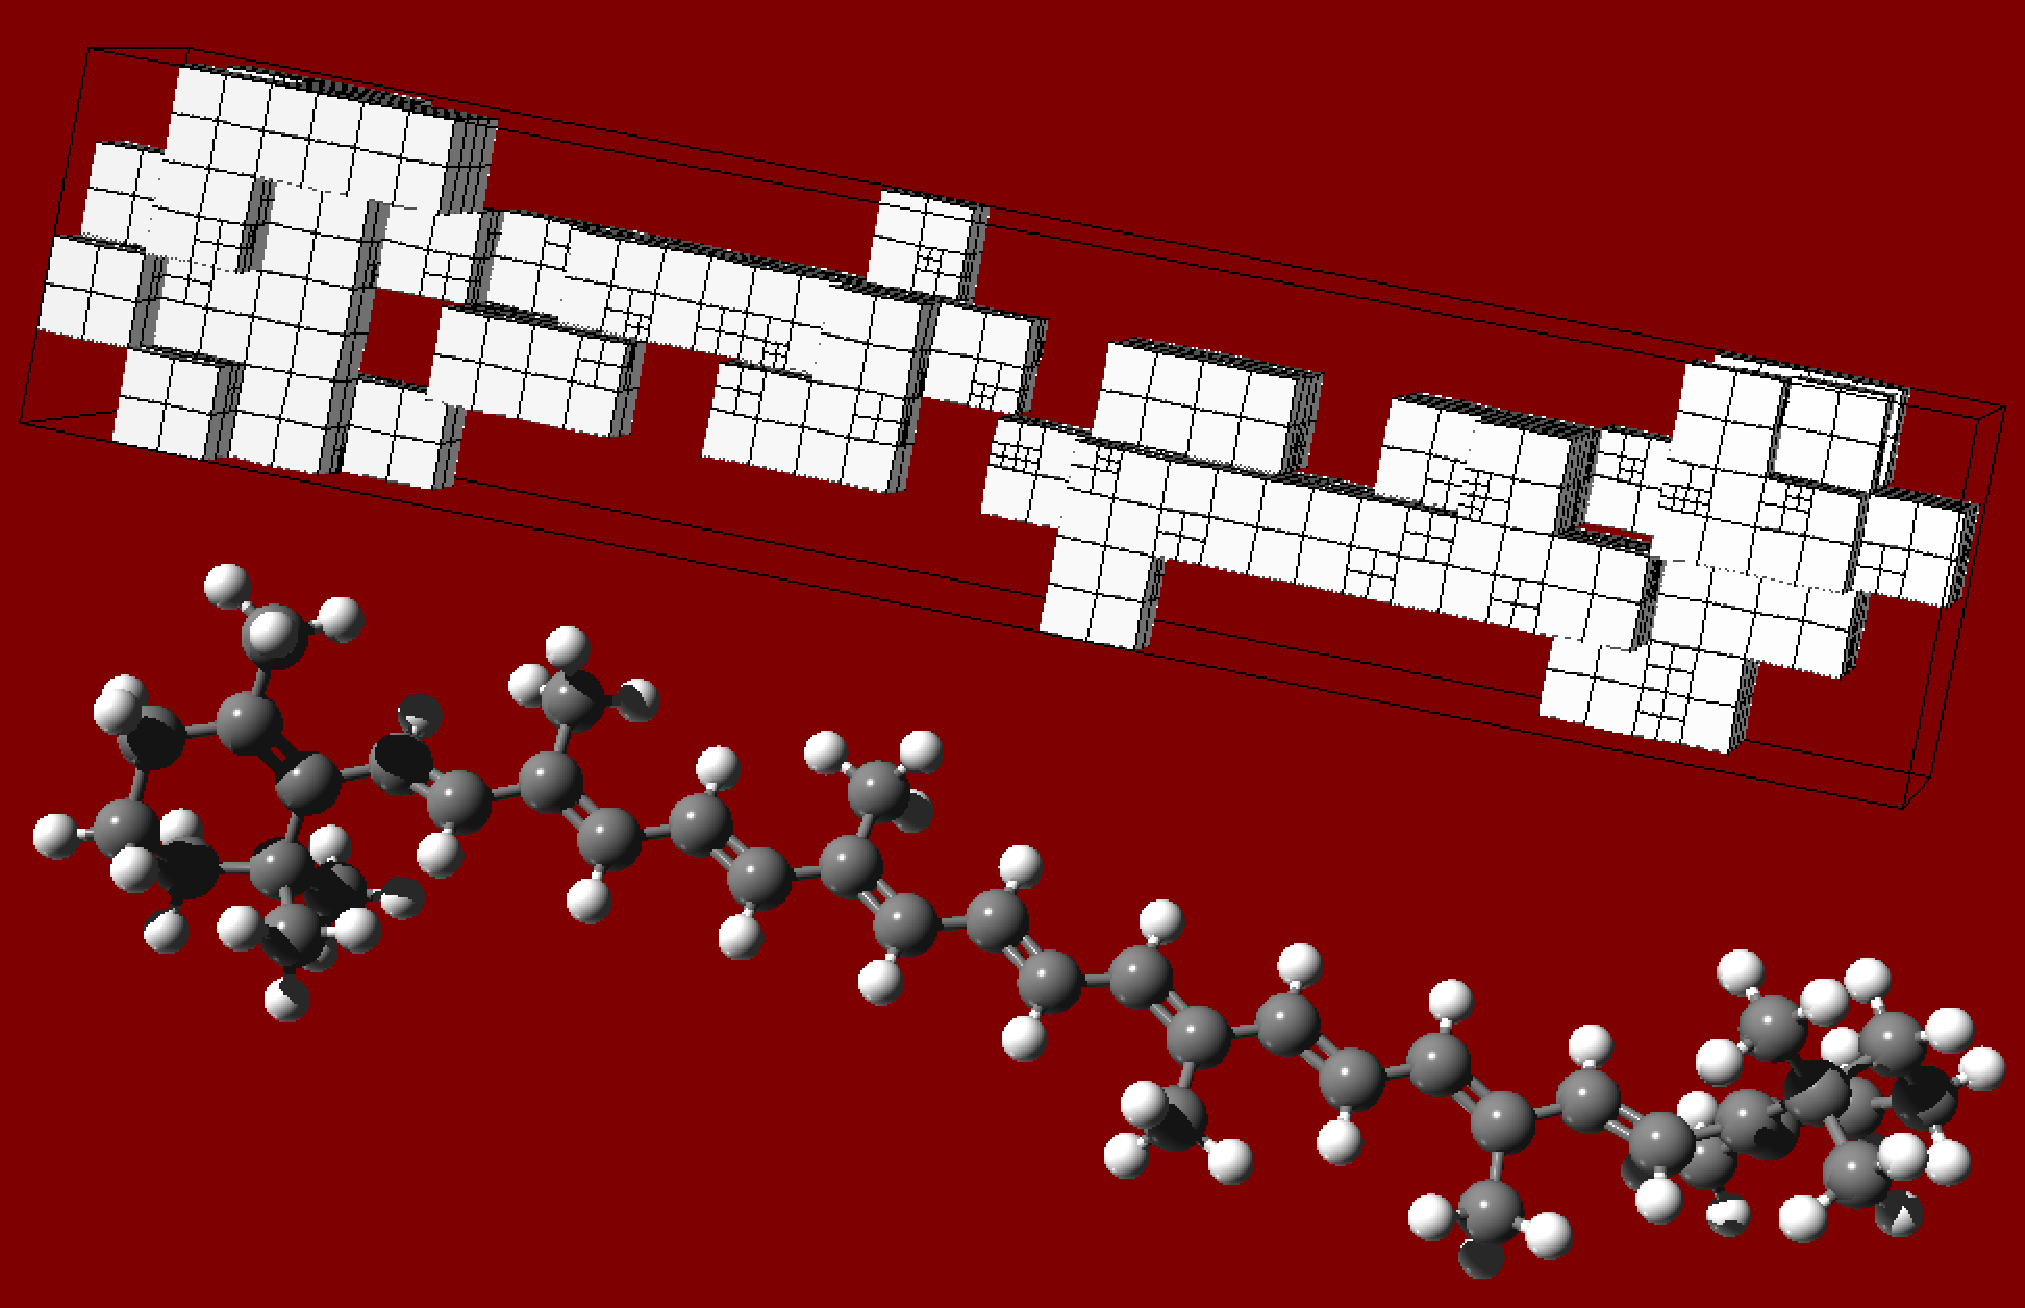
\includegraphics[scale=0.2]{figures/adapGrid.pdf}
    \end{center}
\end{frame}

%\begin{frame}
%    \frametitle{Functions in the MW basis}
%    \only<1>{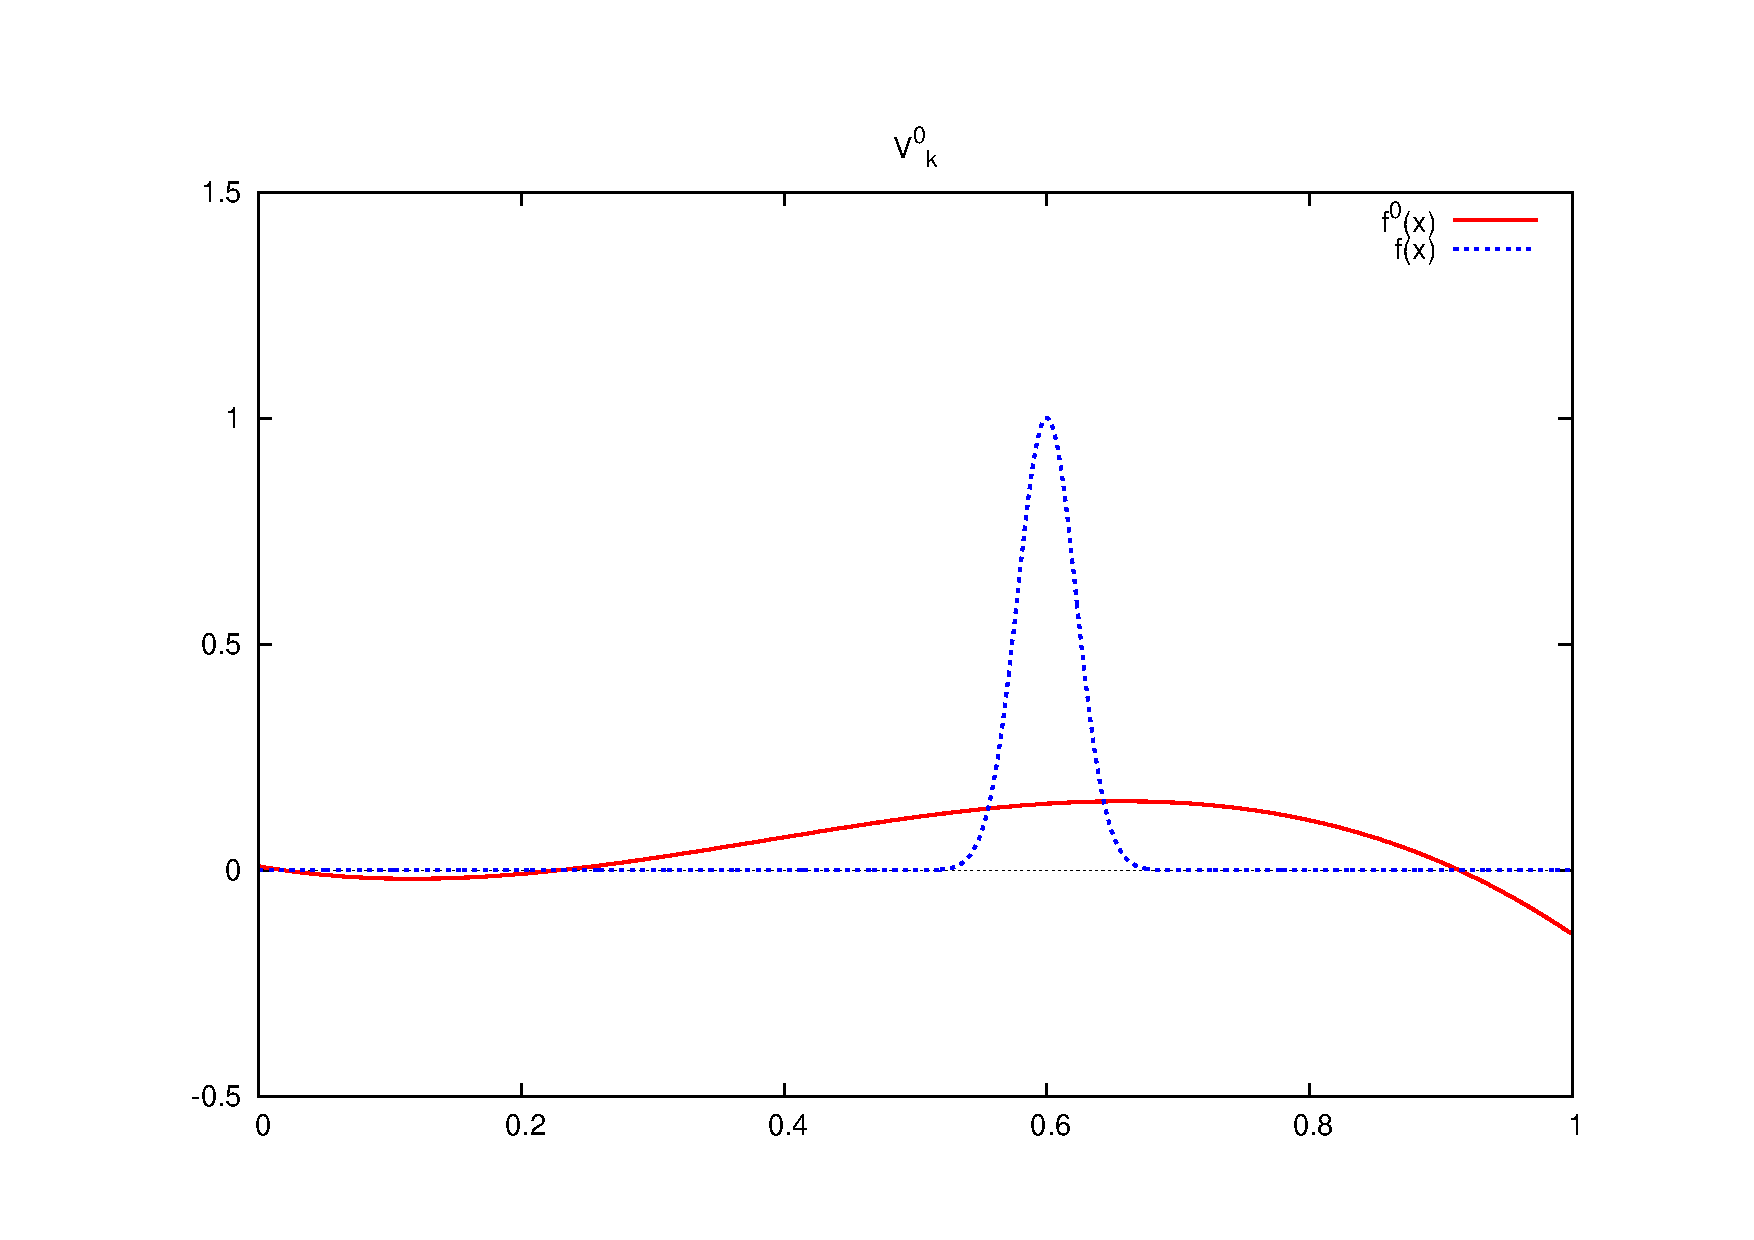
\includegraphics[scale=0.37]{figures/f0.pdf}}
%    \only<2>{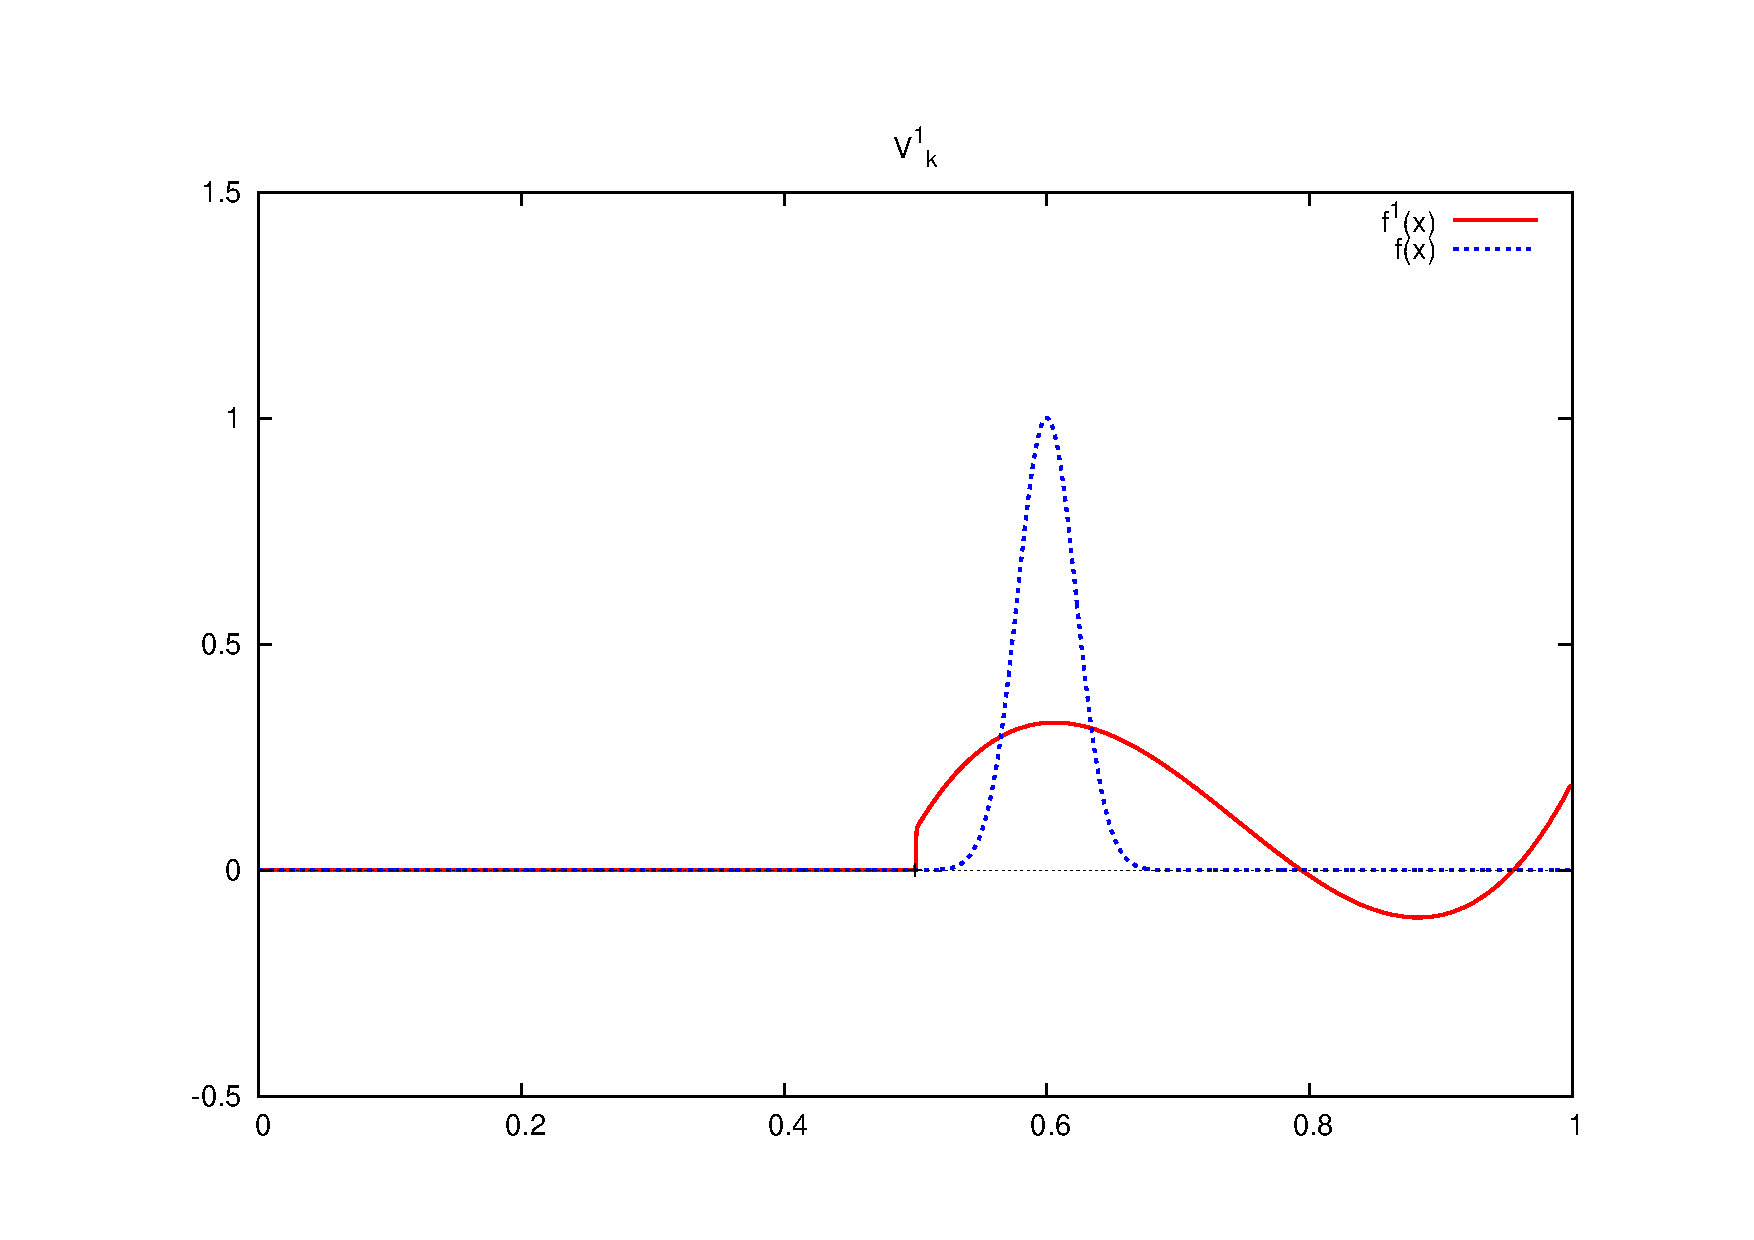
\includegraphics[scale=0.37]{figures/f1.pdf}}
%    \only<3>{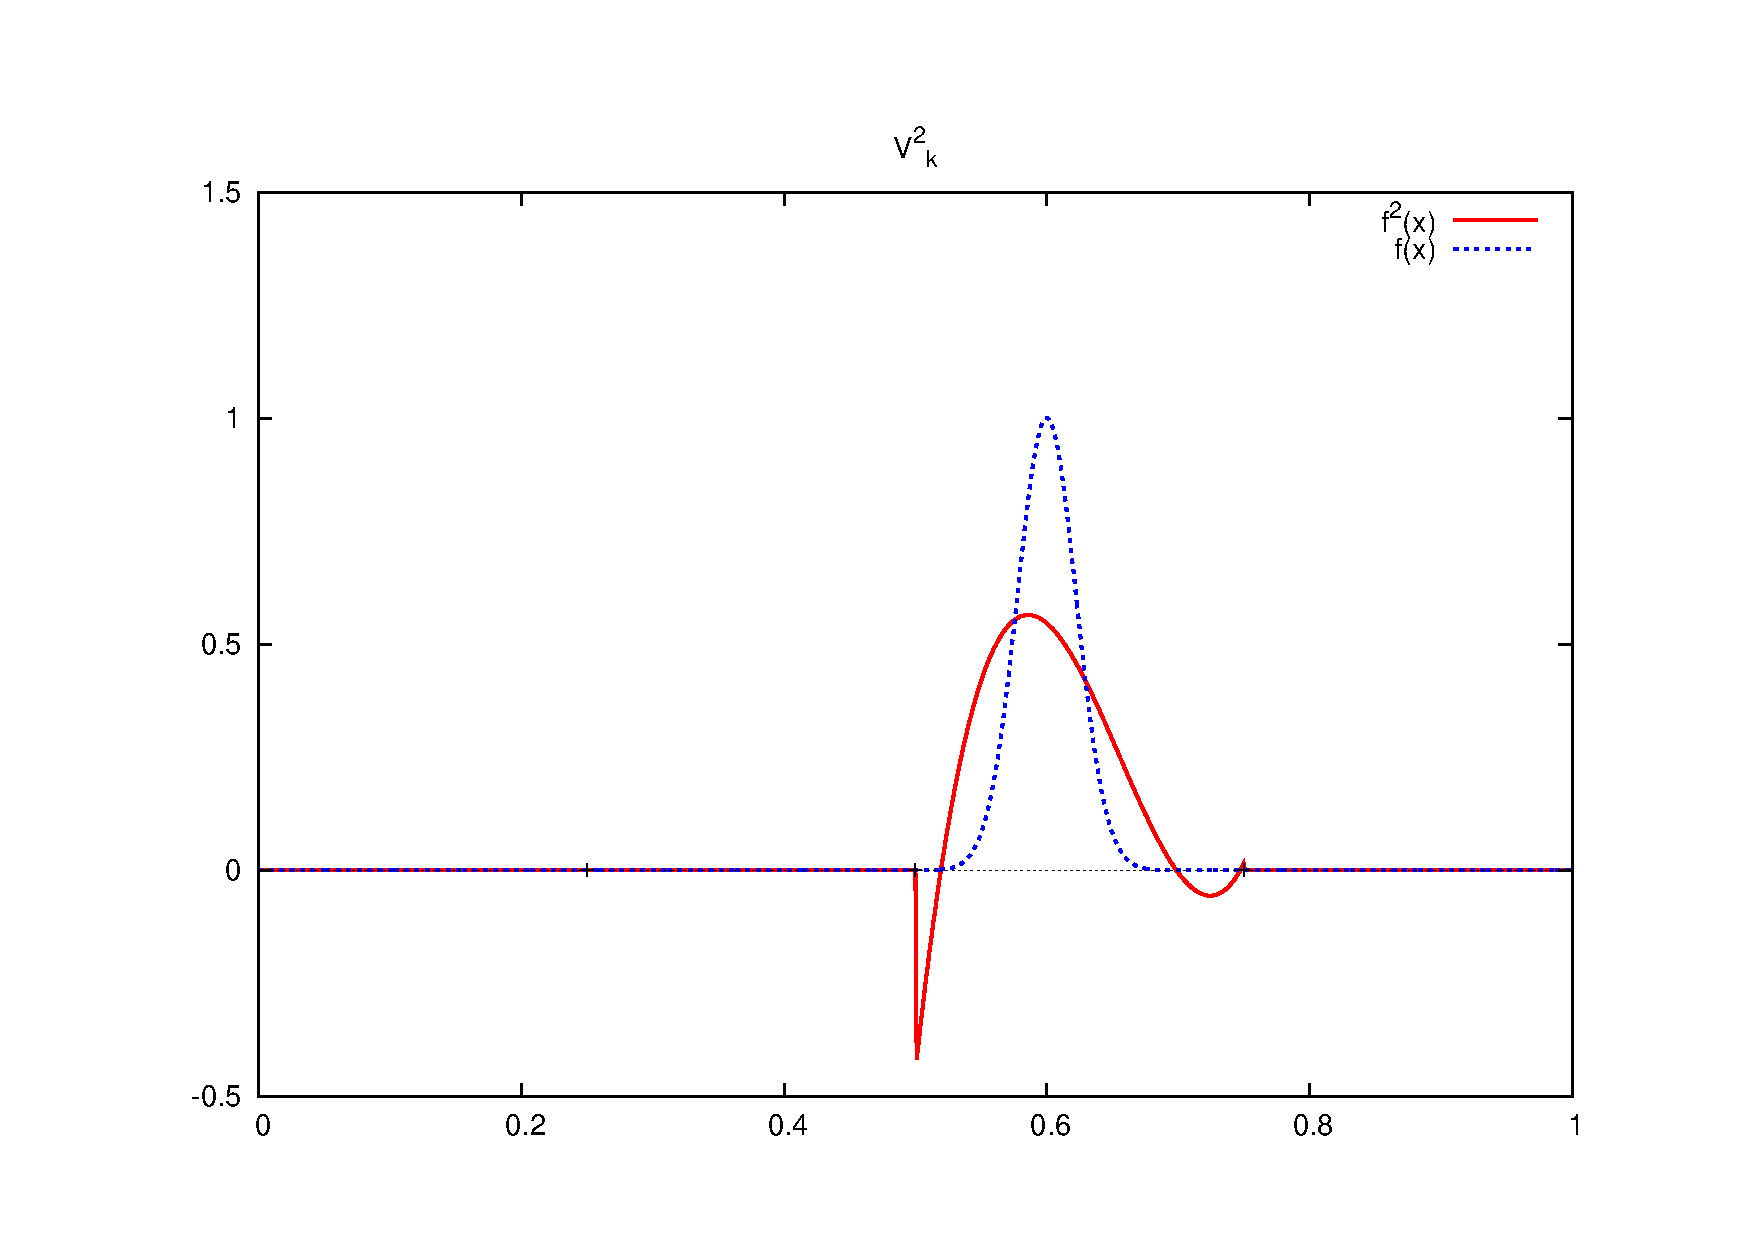
\includegraphics[scale=0.37]{figures/f2.pdf}}
%    \only<4>{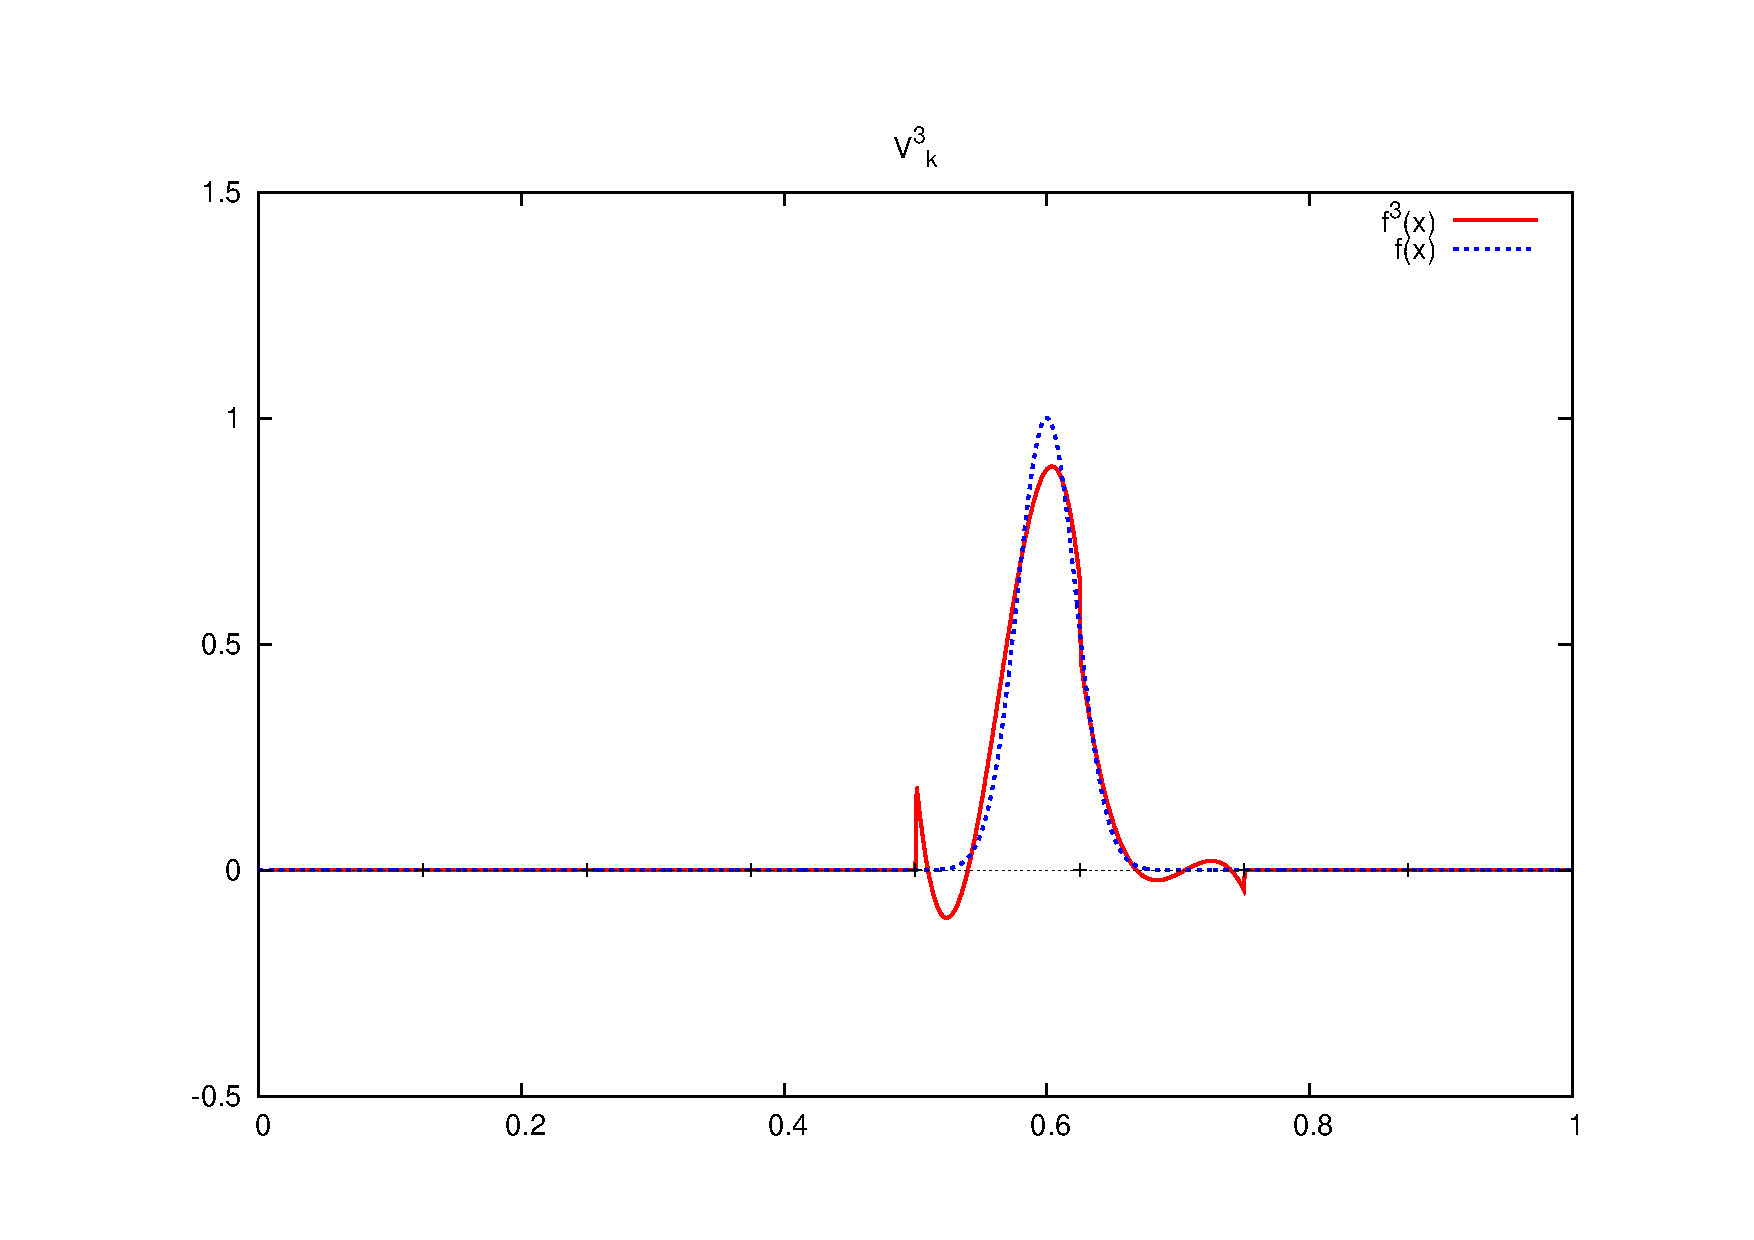
\includegraphics[scale=0.37]{figures/f3.pdf}}
%    \only<5>{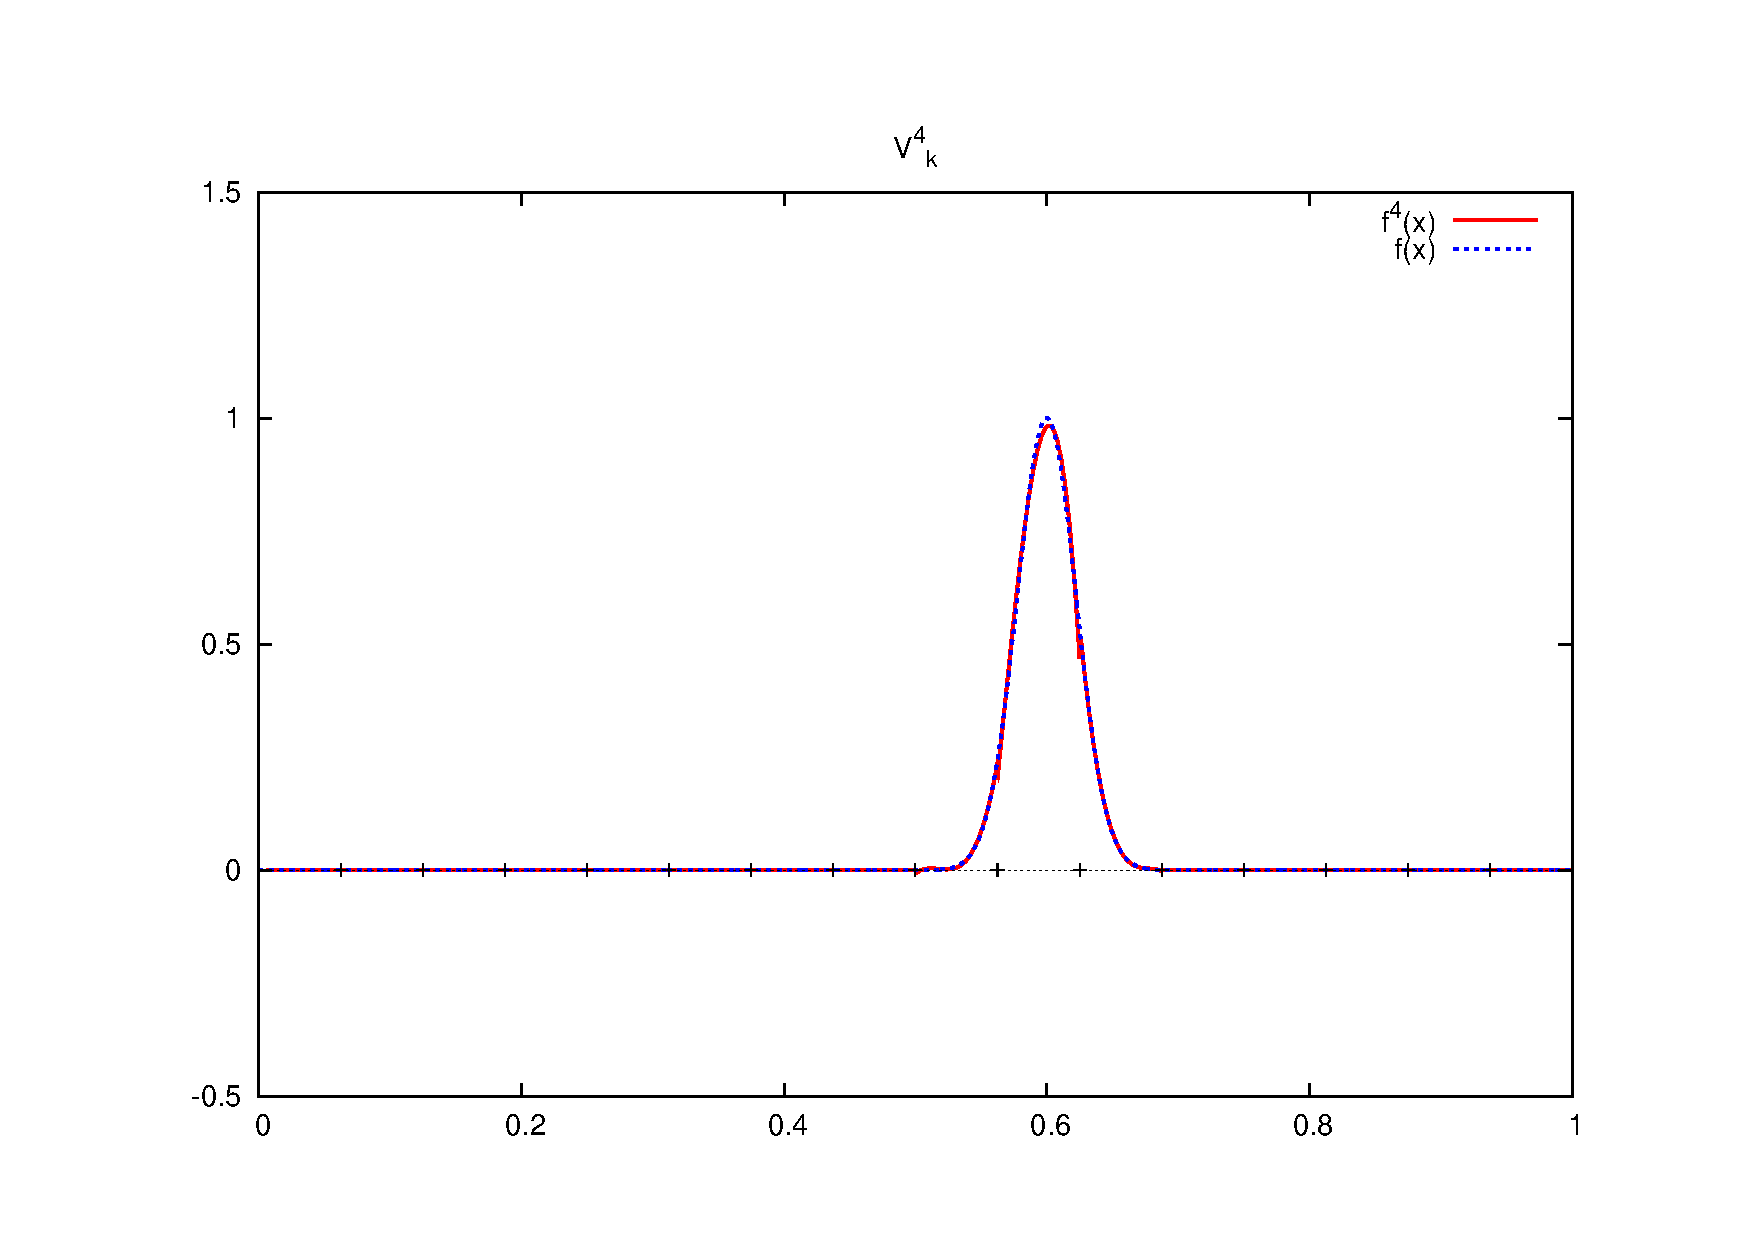
\includegraphics[scale=0.37]{figures/f4.pdf}}
%    \only<6>{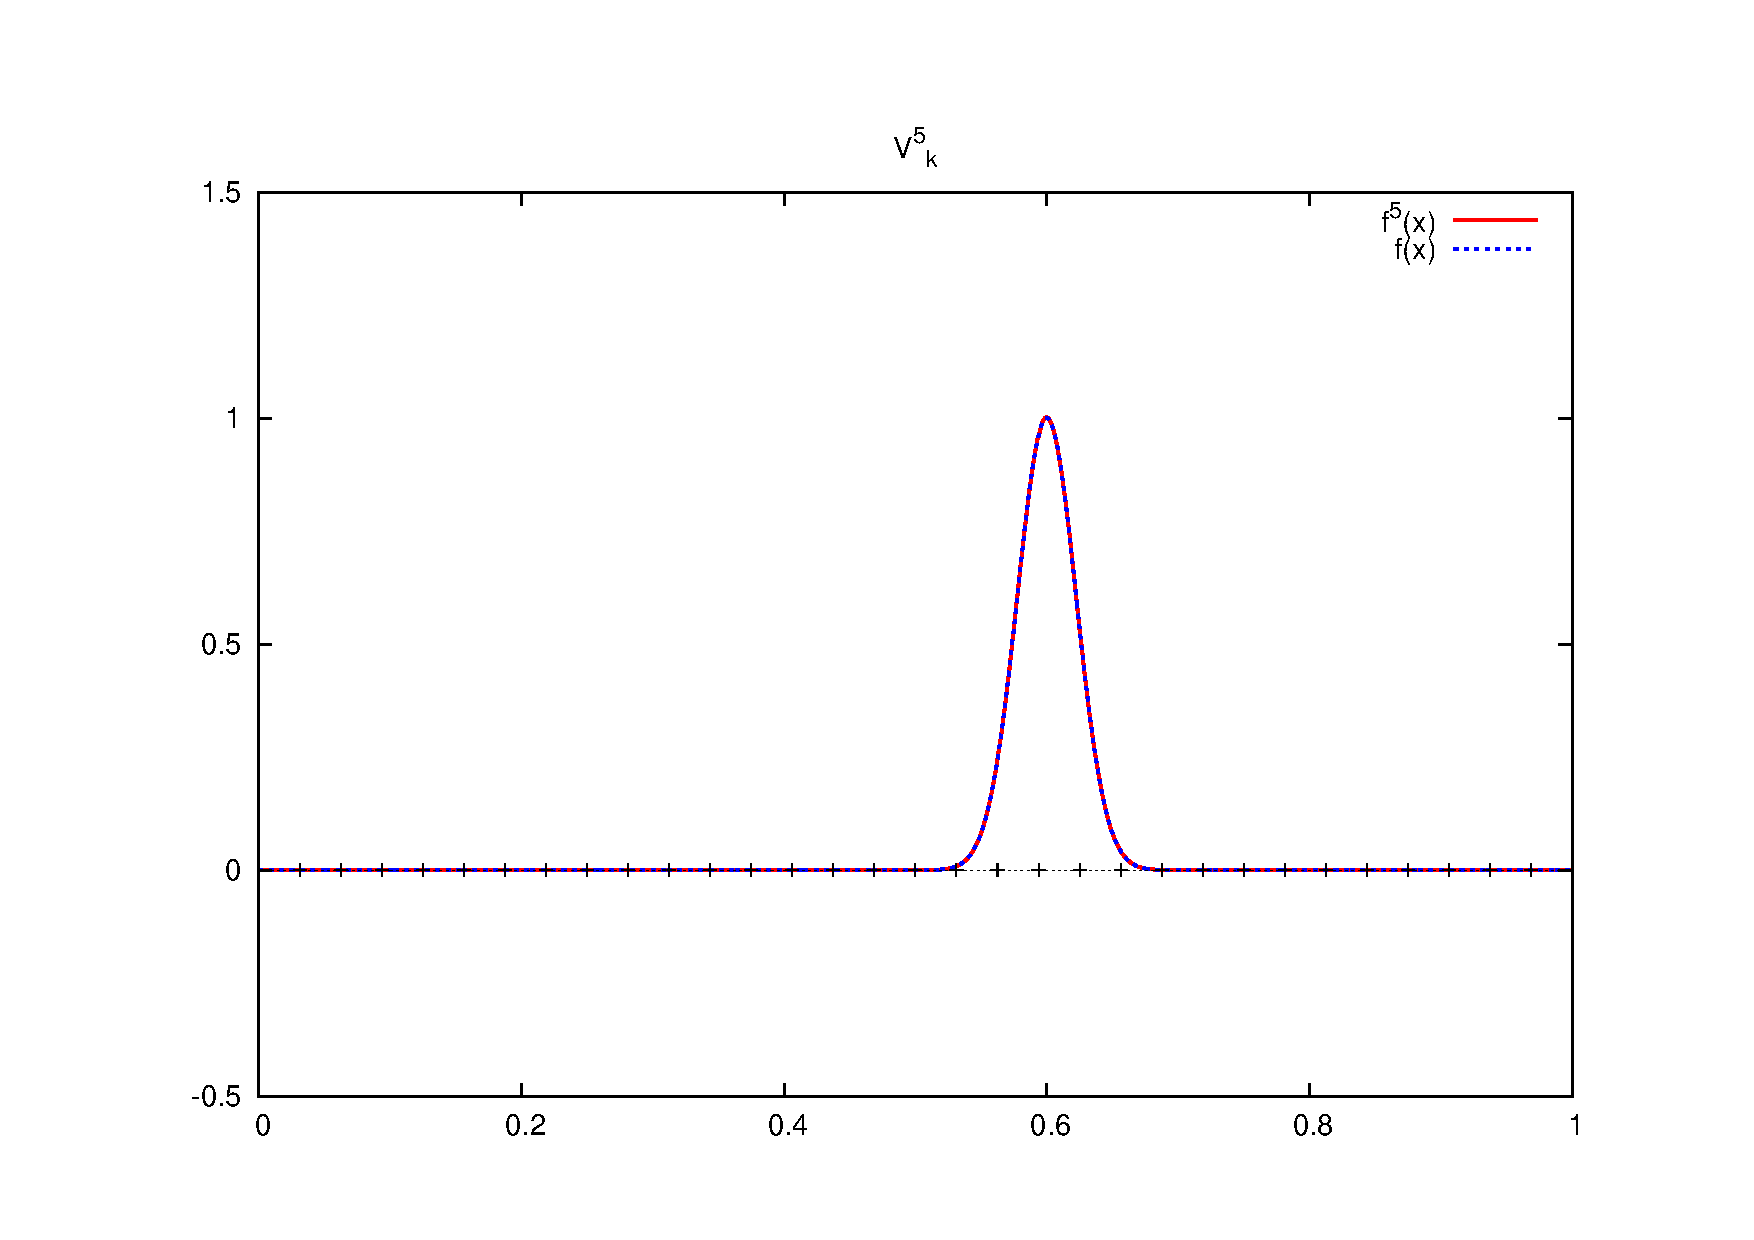
\includegraphics[scale=0.37]{figures/f5.pdf}}
%\end{frame}

\begin{frame}
    \frametitle{Operators in the MW basis}
    MW basis well suited for applying integral operators
    \begin{equation}
	\nonumber
	g(\boldsymbol{r}) = \int K(\boldsymbol{r} - \boldsymbol{r'}) 
	    f(\boldsymbol{r'}) d\boldsymbol{r'}
    \end{equation}
    which have been highly optimized and parallelized, and are linear scaling
    \ \\
    \ \\
    \pause
    \begin{columns}
    \begin{column}{.48\textwidth}
    \begin{itemize}
	\item Poisson kernel (electrostatics)
	    \ \\
	    \ \\
	    \ \\
	\item Bound State Helmholtz (BSH) kernel (Kohn-Sham equations)
	    \ \\
	    \ \\
	    \ \\
	\item Derivative kernel
    \end{itemize}
    \end{column}
    \begin{column}{.48\textwidth}
    \ \\
    \begin{equation}
	\nonumber
	\scriptsize
	P(\boldsymbol{r}-\boldsymbol{r}') = 
	    \frac{1}{4\pi}\ \frac{1}{|\boldsymbol{r}-\boldsymbol{r}'|}
    \end{equation}
    \ \\
    \ \\
    \begin{equation}
	\nonumber
	\scriptsize
	H^{\mu}(\boldsymbol{r}-\boldsymbol{r}') = \frac{1}{4\pi}\ 
	    \frac{e^{-\mu |\boldsymbol{r}-\boldsymbol{r}'|}}{|\boldsymbol{r}-\boldsymbol{r}'|}
    \end{equation}
    \ \\
    \ \\
    \begin{equation}
	\nonumber
	\scriptsize
	D_x(x-x') = \frac{d}{dx} \delta(x - x')
    \end{equation}
    \end{column}
    \end{columns}
\end{frame}

\begin{frame}
	\frametitle{DFT in the MW basis}
	Kohn-Sham equations for orbitals $\phi_i$ of energy $\epsilon_i$
	\begin{align}
		\nonumber
		\big[-\frac{1}{2}\nabla^2 + V_{eff}(\boldsymbol{r})\big]
		\phi_i(\boldsymbol{r}) =&\ \epsilon_i \phi(\boldsymbol{r})\ \ \ \ \ \ \ \ \ \ \ \ 
		\ \ \ \ \ \ \ \ \ \ \ \ \ \ \mu_i = \sqrt{-2\epsilon_i}\\
		\nonumber
		\ & \ \\
		\nonumber
		\big[-\nabla^2 + \mu_i^2\big]\phi_i(\boldsymbol{r}) =&\ 
		    -2\ V_{eff}(\boldsymbol{r})\ \phi_i(\boldsymbol{r})\\
		\nonumber
		\phi_i(\boldsymbol{r}) =&\ -2\int H^{\mu_i}(\boldsymbol{r}-\boldsymbol{r}')\
		    \Big[V_{eff}(\boldsymbol{r}')\ \phi_i(\boldsymbol{r}')\Big] d\boldsymbol{r}'
		%\nonumber
		%\phi(\boldsymbol{r}) =&\ \hat{H} \Big[V_{eff}(\boldsymbol{r}')\ 
		%    \phi(\boldsymbol{r}')\Big]
	\end{align}
	\ \\
	\ \\
	using the BSH Green's kernel.\\
	\ \\
	\pause
	Solved self-consistently by straightforward iteration\\
	\begin{equation}
	    \nonumber
	    \phi^{n+1}_i(\boldsymbol{r}) =\ -2\int H^{\mu^n_i}(\boldsymbol{r}-\boldsymbol{r}')\
		\Big[V^n_{eff}(\boldsymbol{r}')\ \phi^n_i(\boldsymbol{r}')\Big] d\boldsymbol{r}'
	\end{equation}
	\ \\
	\ \\
	\tiny \it{M. H. Kalos; "Monte Carlo calculations of the ground state of three- and 
	    four-body nuclei", Physical Review (1962)}
\end{frame}

%\begin{frame}
%	\frametitle{Power iteration and Newton's method}
%	The series
%	\begin{equation}
%		\nonumber
%		A\phi, A^2\phi, A^3\phi, \dots, A^n\phi
%	\end{equation}
%	\ \\
%	\ \\
%	will converge to the egenfunction of A with the highest eigenvalue 
%	(absolute value).
%	\ \\
%	\ \\
%	Straightforward power iteration of the integral operator gives
%	\begin{equation}
%		\nonumber
%		\phi^{n+1} = \hat{H}\big[V_{eff}\phi^n\big]
%	\end{equation}
%	We search the root of the following function
%	\begin{equation}
%		\nonumber
%		f(\phi) = \hat{H}\big[V_{eff}\phi\big] -\phi
%	\end{equation}
%	Newton's method for finding roots
%	\begin{align}
%		\nonumber
%		\phi^{n+1} 
%		&= \phi^n - \big[J(\phi^n)\big]^{-1} f(\phi^n)\\
%		\nonumber
%		&= \phi^n - \big[J(\phi^n)\big]^{-1}
%		\big(\hat{H}\big[V_{eff}\phi^n\big] - \phi^n\big)
%	\end{align}
%	So the direct power iteration is an "inexact" Newton method where we
%	approximate the Jacobian $J(\phi^n) \approx -1$.
%\end{frame}
%
%\begin{frame}
%	\frametitle{Krylov Accelerated Inexact Newton (KAIN)}
%	We want to use the history of the orbital
%	\begin{equation}
%		\nonumber
%		\phi^0, \phi^1, \dots, \phi^n
%	\end{equation}
%	and its residual
%	\begin{equation}
%		\nonumber
%		f(\phi^0), f(\phi^1), \dots, f(\phi^n)
%	\end{equation}
%	\ \\
%	\ \\
%	to find a better approximation of the Jacobian.
%	\ \\
%	\ \\
%	The new iterative step is then expanded in the Krylov history
%	\begin{equation}
%		\nonumber
%		\phi^{n+1} = \phi^{n} + \delta\phi^{n}
%	\end{equation}
%	\begin{equation}
%		\nonumber
%		\delta\phi^n = \sum_i c_i\big[\phi^i-\phi^n\big] - 
%		\sum_i c_i\big[f(\phi^i) - f(\phi^n)\big] - f(\phi^n)
%	\end{equation}
%	where the coefficients $c_i$ are computed by projection.\\
%	\ \\
%	\tiny \it{R. J. Harrison; "Krylov subspace accelerated inexact Newton method for linear
%	    and nonlinear equations", JCC (2004)}
%\end{frame}

\begin{frame}
	\frametitle{Hydrogen ground state}
	Effective potential is just nuclear attraction
	\begin{equation}
		\nonumber
		V_{eff} = V_{nuc}(\boldsymbol{r}) = 
		-\sum_i \frac{Z_i}{|\boldsymbol{r}-\boldsymbol{R}_i|}
	\end{equation}
	\ \\
	Ground state is obtained through iterative solution of
	\begin{equation}
	    \nonumber
	    \phi^{n+1}(\boldsymbol{r}) =\ -2\int H^{\mu^n}(\boldsymbol{r}-\boldsymbol{r}')\
		\Big[V_{nuc}(\boldsymbol{r}')\ \phi^n(\boldsymbol{r}')\Big] d\boldsymbol{r}'
	\end{equation}
	\pause
	\begin{table}
		\tiny
		\centering
		\begin{tabular}{|r|r@{.}l|r@{.}l@{e}l|r@{.}l@e{l}|
				r@{.}l|r@{.}l@{e}l|r@{.}l@e{l}|}
			\hline
			&
			\multicolumn{8}{c|}{Power iteration}&
			\multicolumn{8}{c|}{Krylov accelerated}\\
			Iteration&
			\multicolumn{2}{c|}{$E$}&
			\multicolumn{3}{c|}{$\Delta E$}&
			\multicolumn{3}{c|}{$\Delta \phi$}&
			\multicolumn{2}{c|}{$E$}&
			\multicolumn{3}{c|}{$\Delta E$}&
			\multicolumn{3}{c|}{$\Delta \phi$}\\
			\hline
			 1&-0&49844793&-6&18&-03&6&77&-02&-0&49844793&-6&18&-03&6&77&-02\\
			 2&-0&49964578&-1&19&-03&2&87&-02&-0&50056792&-2&12&-03&2&87&-02\\
			 3&-0&49991507&-2&69&-04&1&34&-02&-0&49982342& 7&44&-04&1&69&-03\\
			 4&-0&49997918&-6&41&-05&6&53&-03&-0&50012138&-2&98&-04&4&66&-04\\
			 5&-0&49999484&-1&57&-05&3&22&-03&-0&49999713& 1&24&-04&2&27&-04\\
			 6&-0&49999870&-3&87&-06&1&60&-03&-0&49999977&-2&64&-06&3&29&-06\\
			 7&-0&49999967&-9&62&-07&7&99&-04&-0&49999995&-1&80&-07&2&87&-07\\
			 8&-0&49999990&-2&40&-07&3&99&-04&-0&49999999&-3&77&-08&3&40&-08\\
			 9&-0&49999997&-5&96&-08&2&00&-04&
			\multicolumn{2}{c|}{}&\multicolumn{3}{c|}{}&\multicolumn{3}{c|}{}\\
			10&-0&49999998&-1&54&-08&9&98&-05&
			\multicolumn{2}{c|}{}&\multicolumn{3}{c|}{}&\multicolumn{3}{c|}{}\\
			11&-0&49999999&-3&83&-09&4&99&-05&
			\multicolumn{2}{c|}{}&\multicolumn{3}{c|}{}&\multicolumn{3}{c|}{}\\
			\hline
			Exact&-0&50000000&
			\multicolumn{3}{c|}{}&
			\multicolumn{3}{c|}{}&
			-0&50000000&
			\multicolumn{3}{c|}{}&
			\multicolumn{3}{c|}{}\\
			\hline
		\end{tabular}
	\end{table}
	\tiny \it{R. J. Harrison; "Krylov subspace Accelerated Inexact Newton method for linear
	    and nonlinear equations", JCC (2004)}
\end{frame}
%
%\begin{frame}
%	\frametitle{Hydrogen ground state}
%	\only<1>{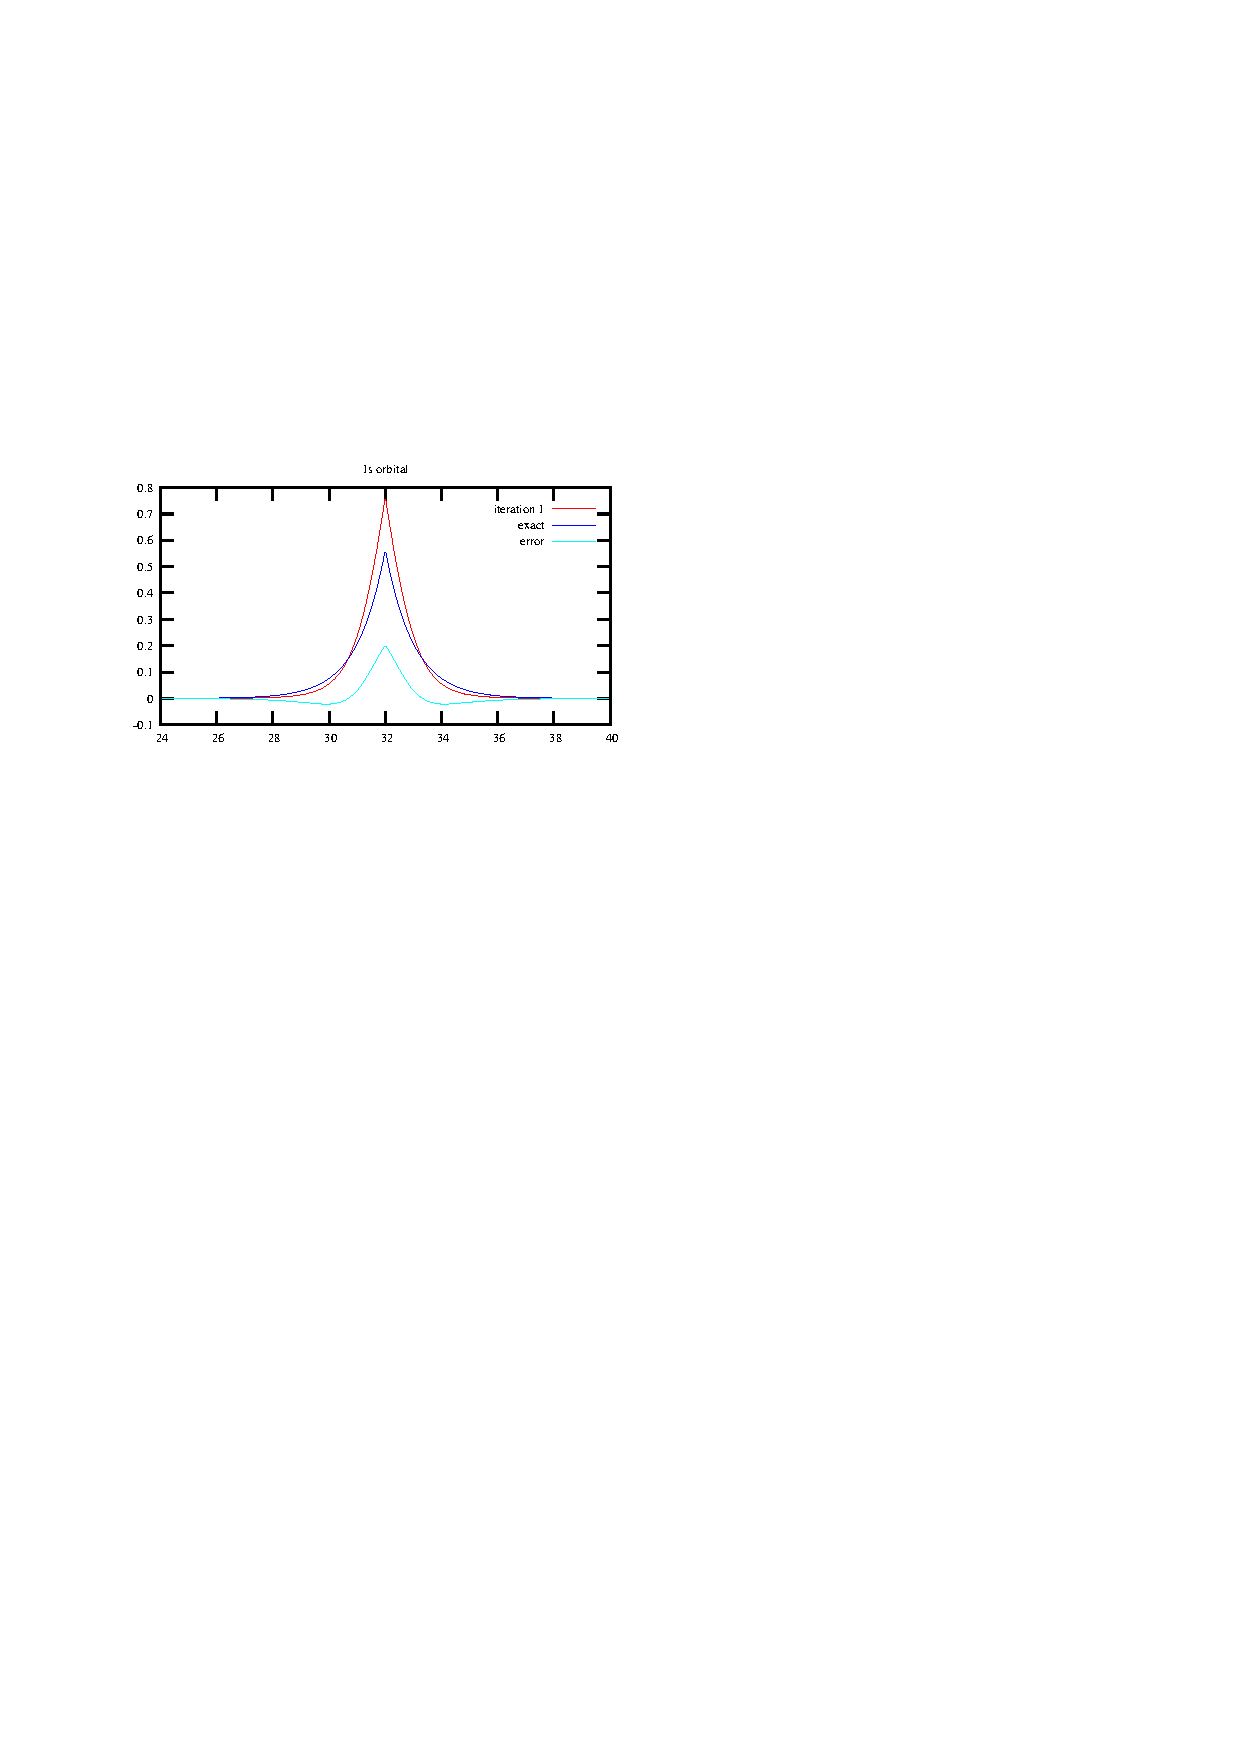
\includegraphics[bb = 50 430 300 640, clip, scale=1.2]{figures/s1Orb_1.pdf}}
%	\only<2>{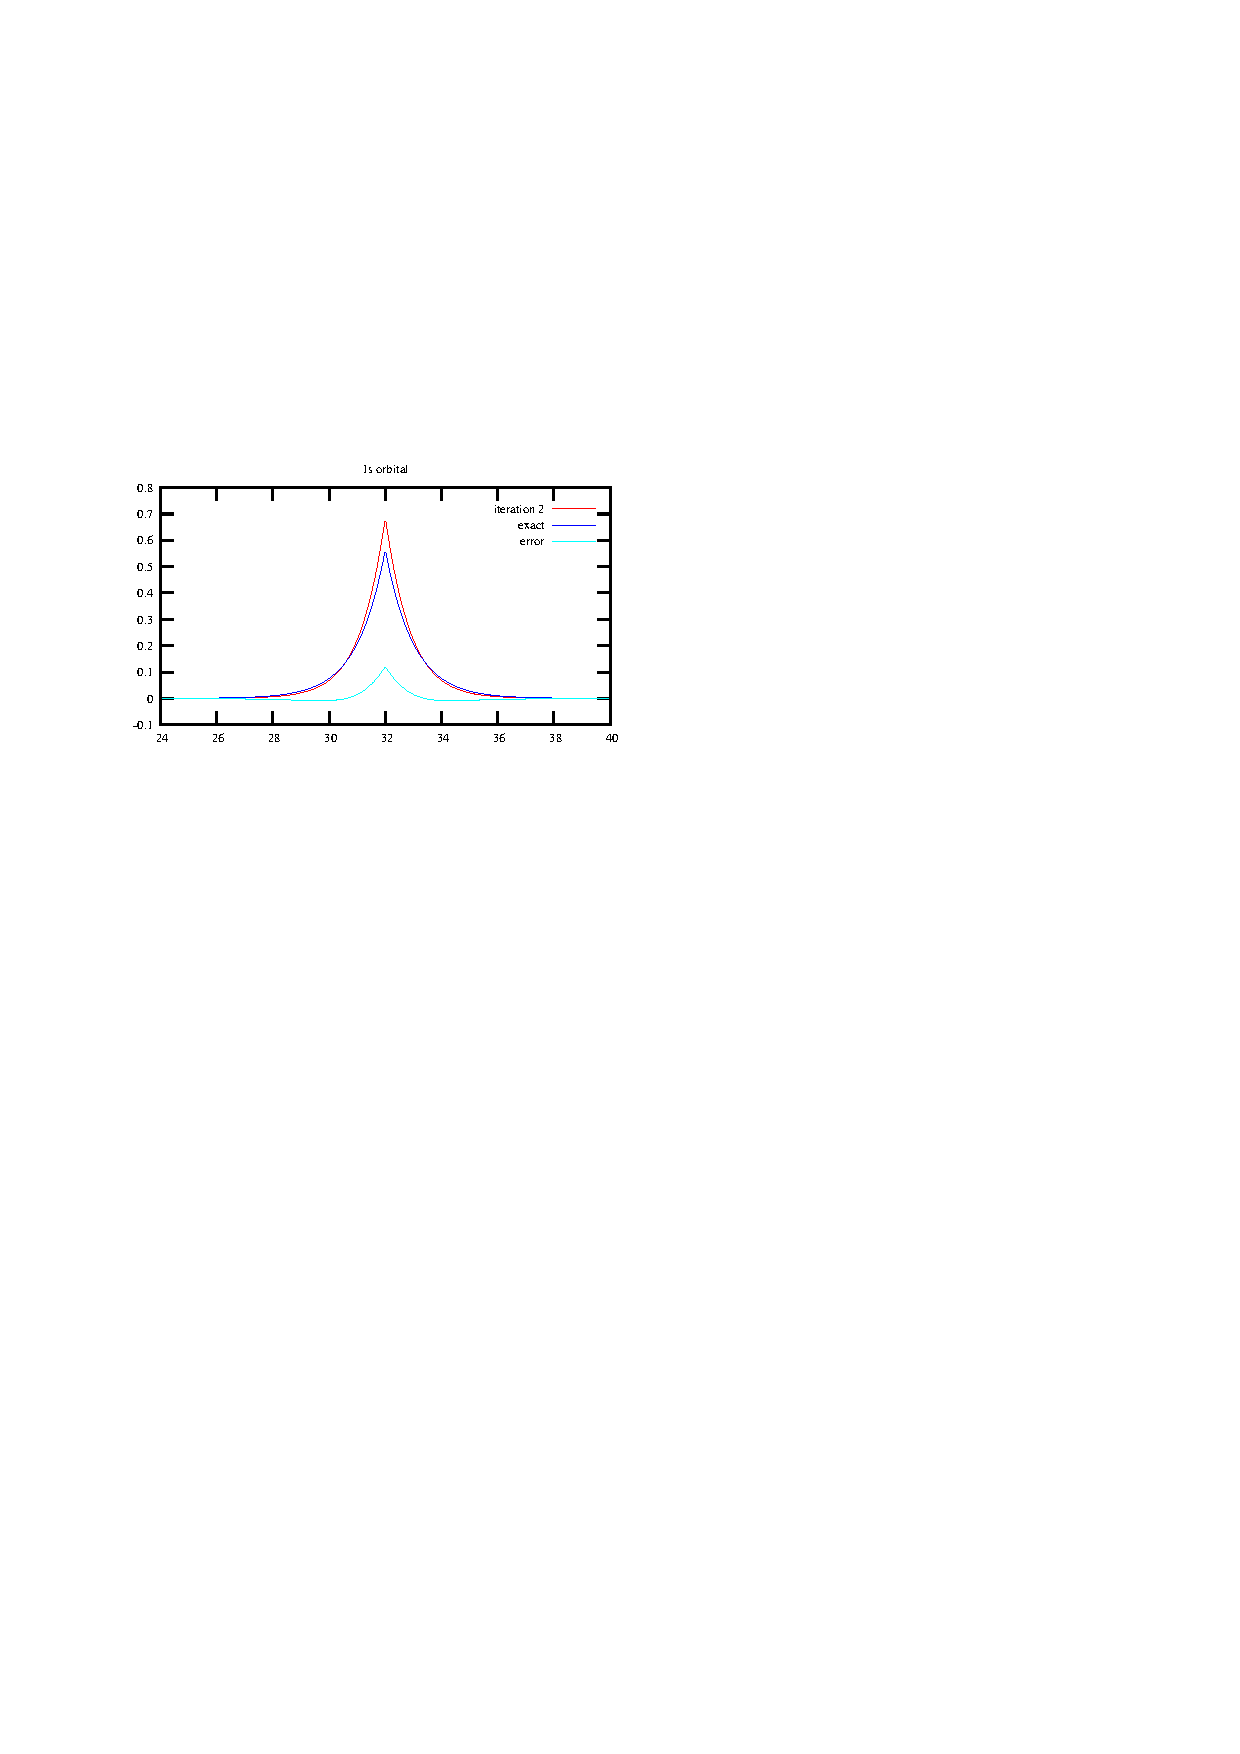
\includegraphics[bb = 50 430 300 640, clip, scale=1.2]{figures/s1Orb_2.pdf}}
%	\only<3>{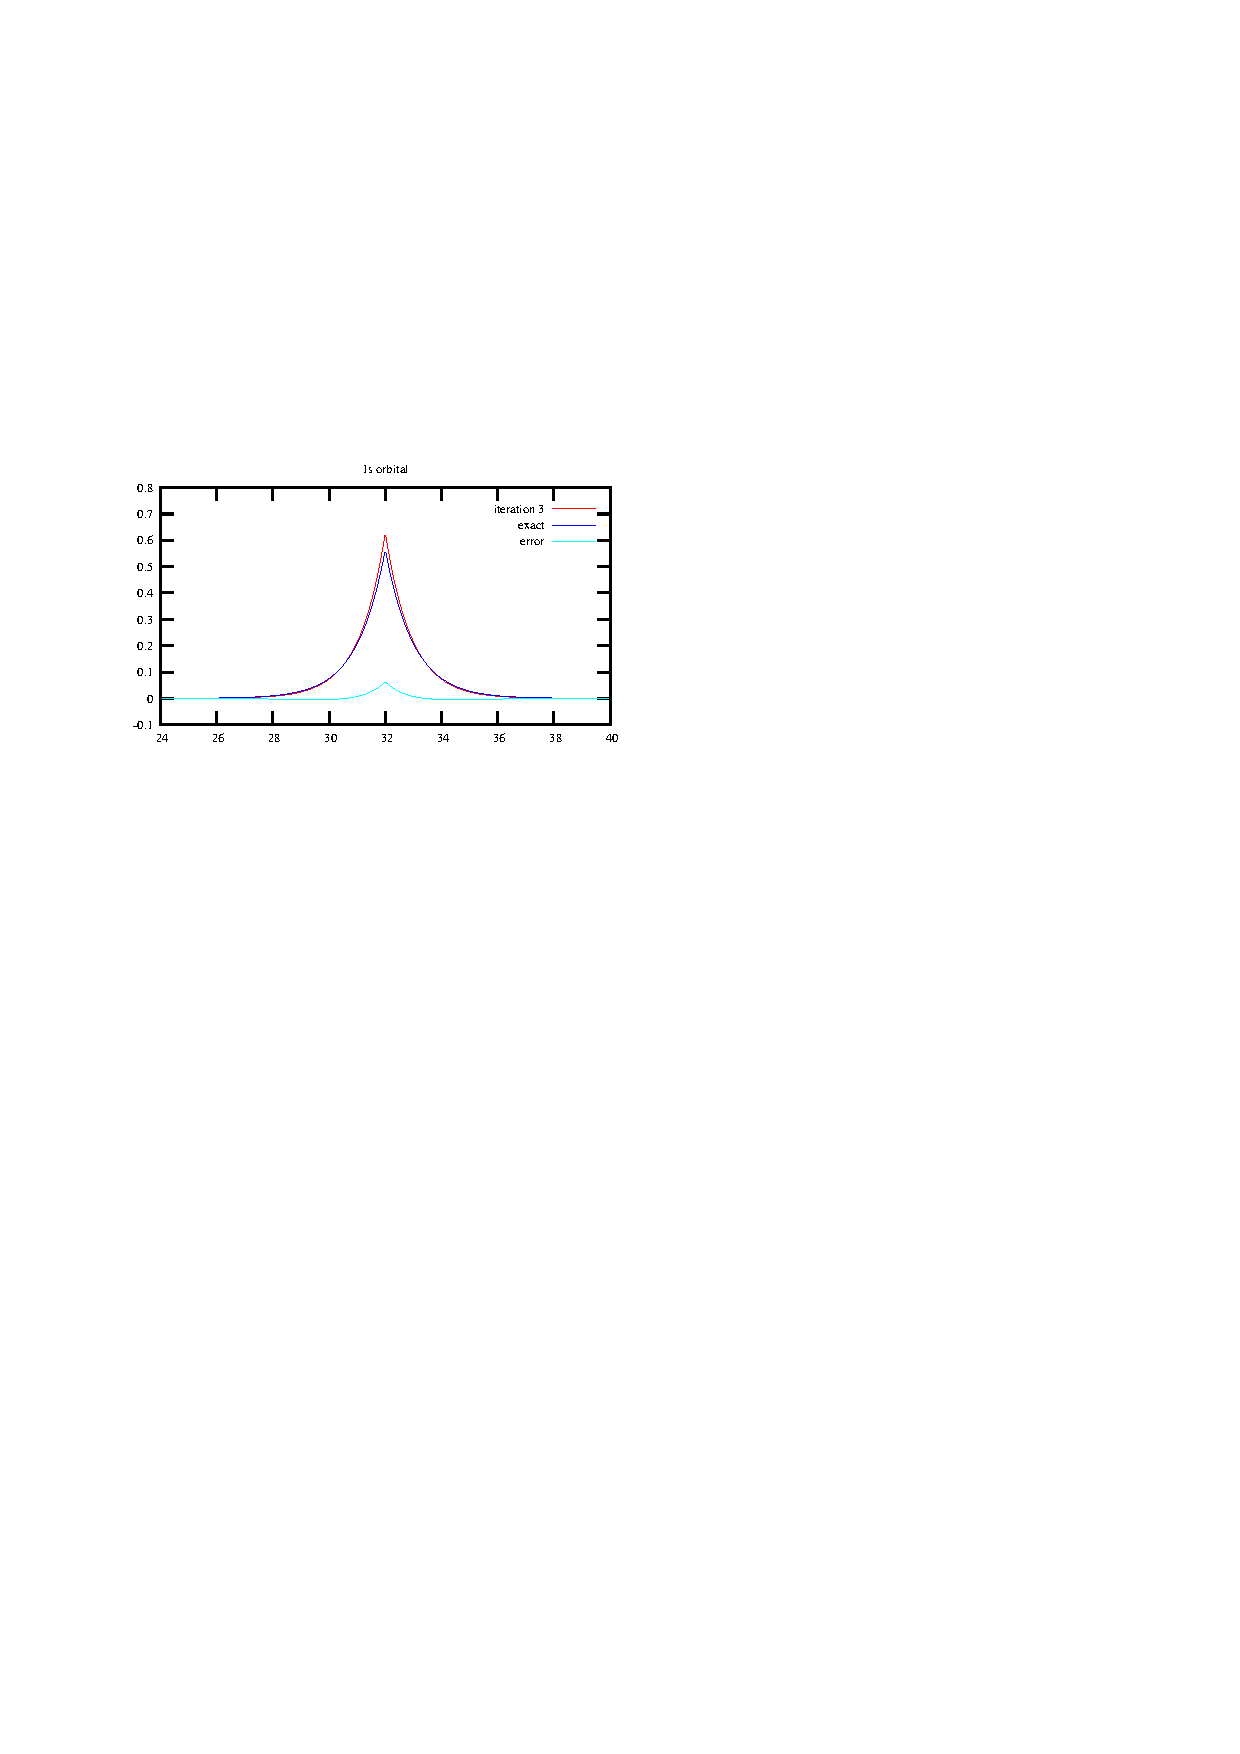
\includegraphics[bb = 50 430 300 640, clip, scale=1.2]{figures/s1Orb_3.pdf}}
%	\only<4>{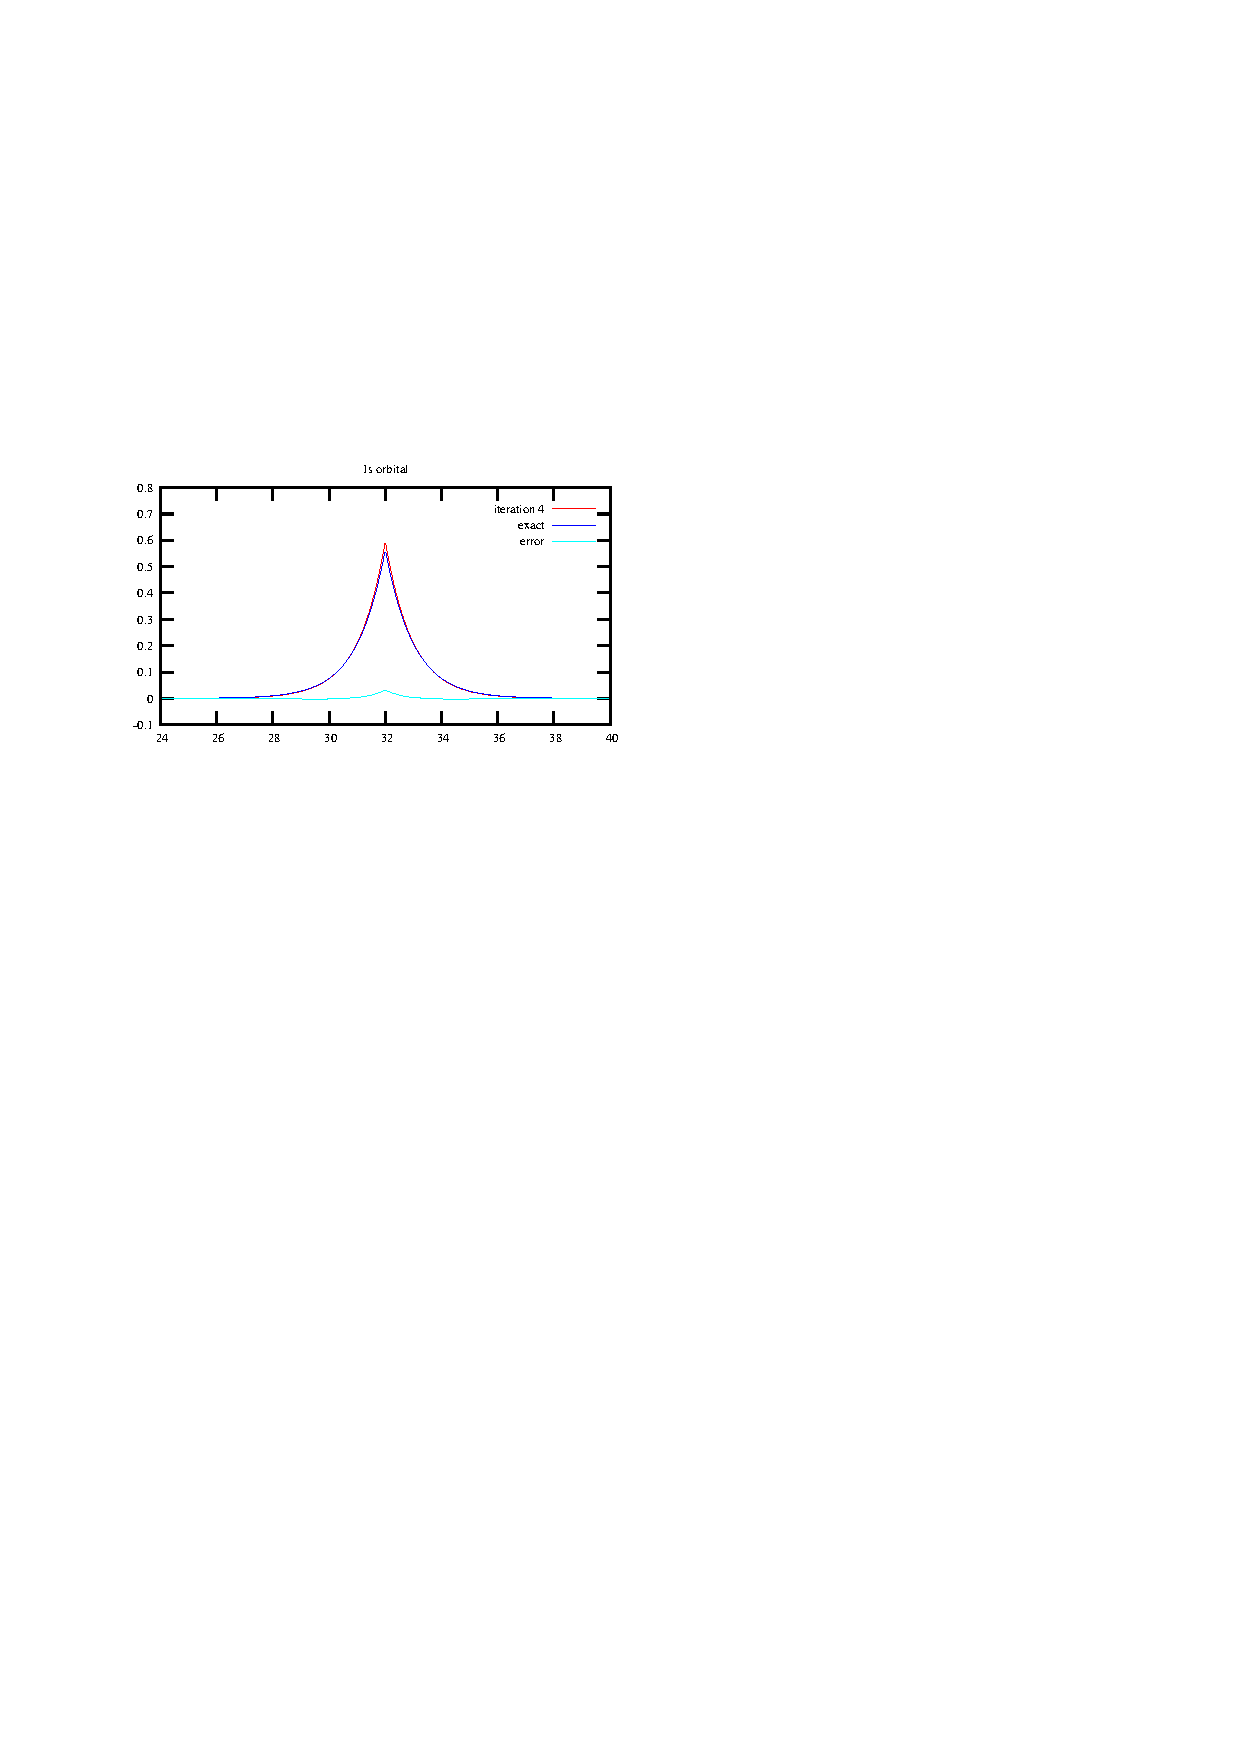
\includegraphics[bb = 50 430 300 640, clip, scale=1.2]{figures/s1Orb_4.pdf}}
%	\only<5>{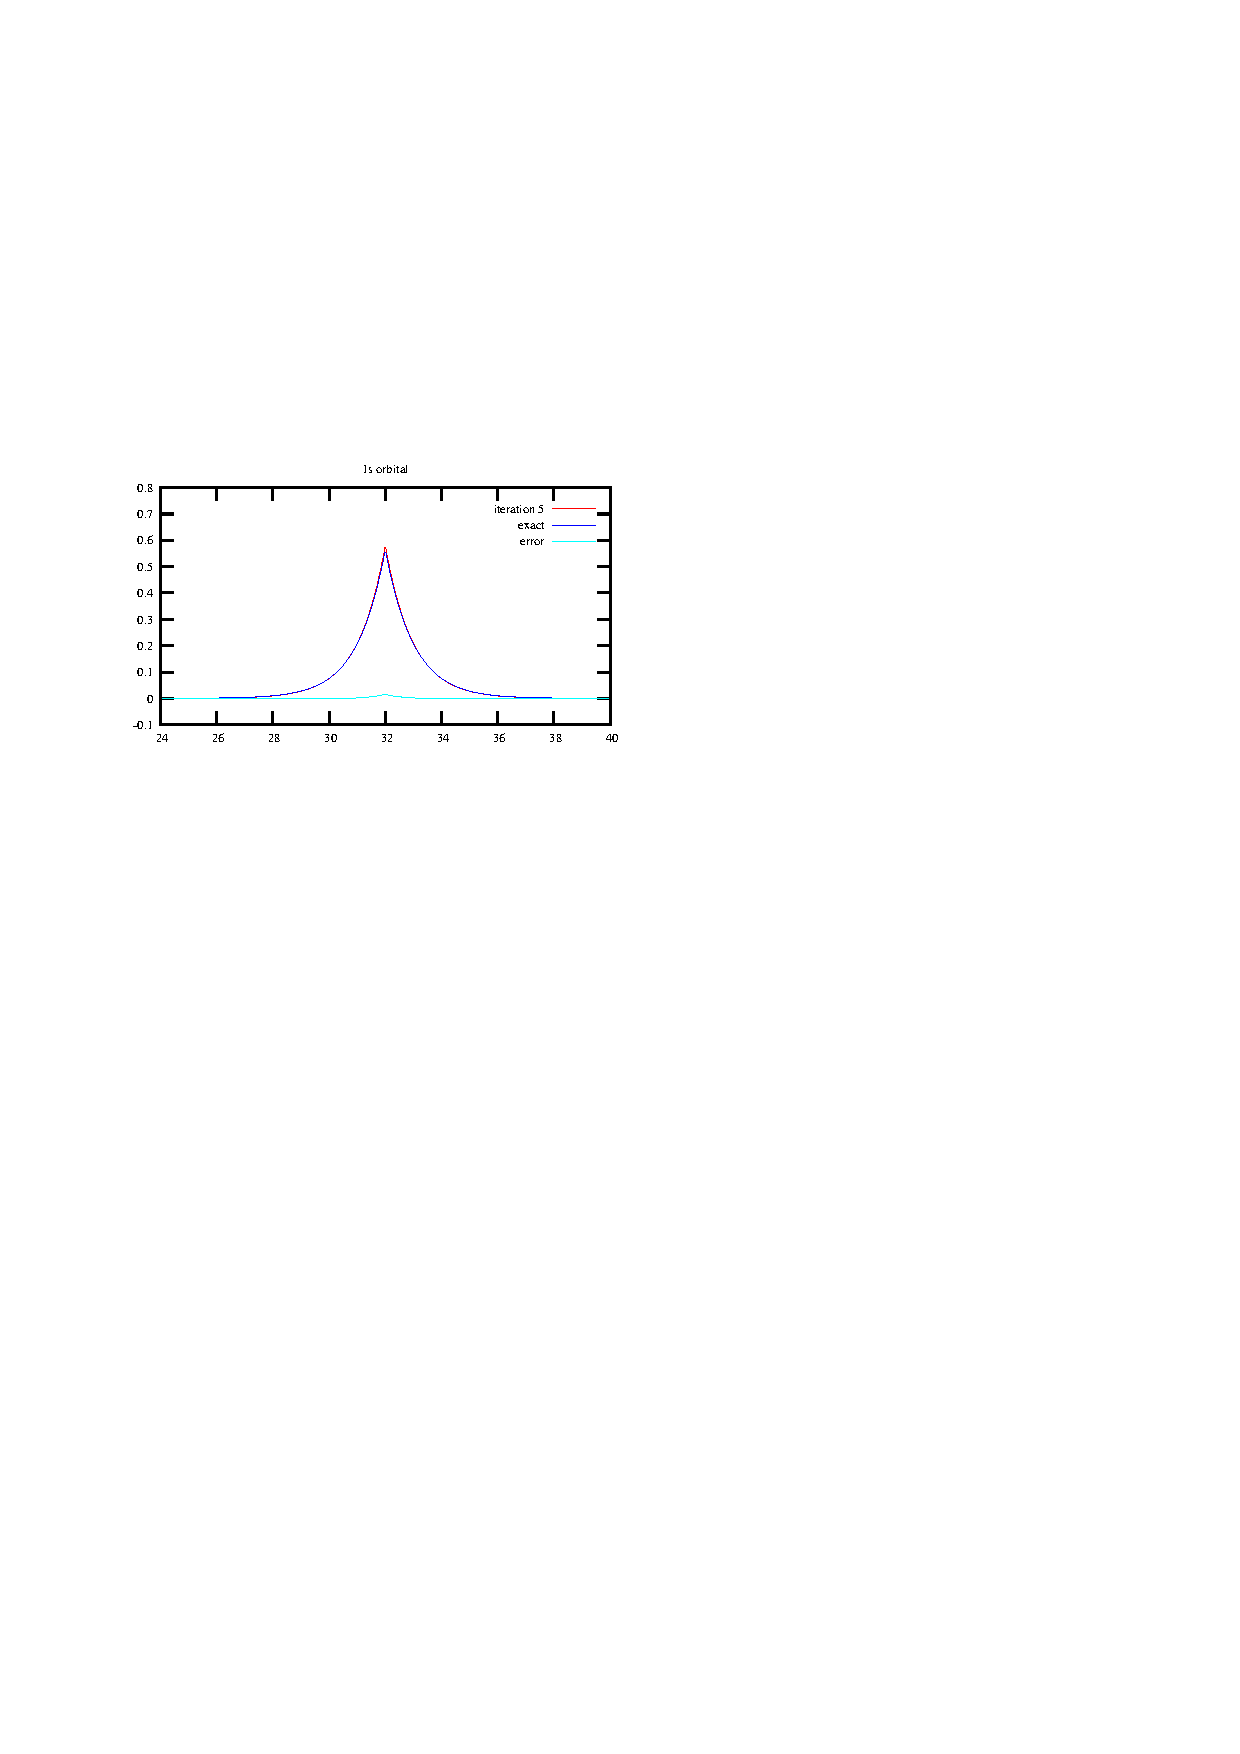
\includegraphics[bb = 50 430 300 640, clip, scale=1.2]{figures/s1Orb_5.pdf}}
%	\only<6>{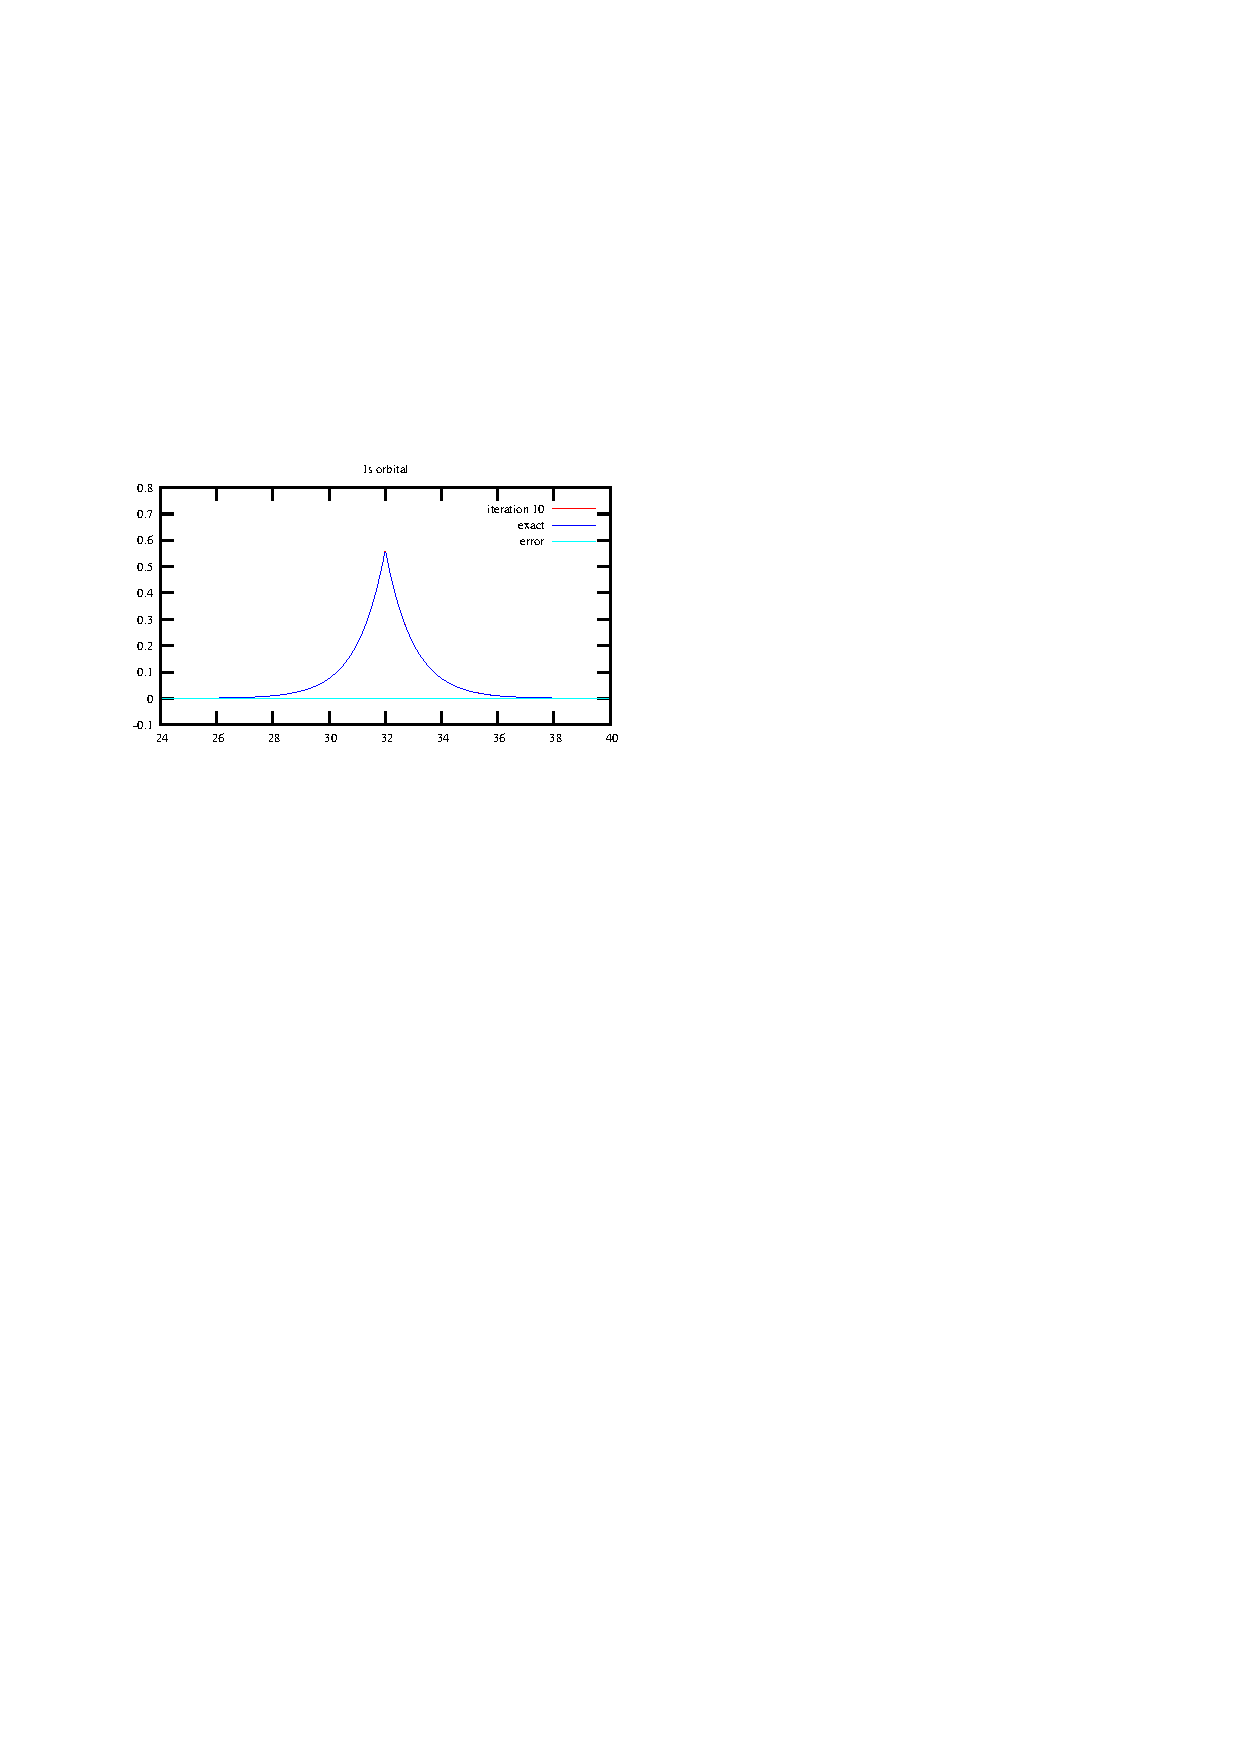
\includegraphics[bb = 50 430 300 640, clip, scale=1.2]{figures/s1Orb_10.pdf}}
%\end{frame}

\begin{frame}
    \frametitle{DFT in the MW basis}
    For many-electron systems in DFT the effective potential is given
    \begin{equation}
	\nonumber
	V_{eff} = V_{nuc} + V_{coul} + V_{xc}
    \end{equation}
    \ \\
    \ \\
    \ \\
    \pause
    The Coulomb potential is given by the Poisson equation 
    \begin{equation}
	\nonumber
	V_{coul}(\boldsymbol{r}) = 
	\int
	P(\boldsymbol{r} - \boldsymbol{r}') \Big[ \rho(\boldsymbol{r}')\Big] d\boldsymbol{r}'
    \end{equation}
    \ \\
    \ \\
    \ \\
    \pause
    The XC potential is given as the functional derivative
    \begin{equation}
	\nonumber
	V_{xc} \ \ \ = \ \ \ \frac{\delta E_{xc}[\rho]}{\delta \rho(\boldsymbol{r})}
	       \ \ \ = \ \ \ \frac{\partial F}{\partial \rho} - 
		    \nabla \frac{\partial F}{\partial \nabla \rho}
    \end{equation}
    which is calculated on its own multiresolution grid using XCFun\\
    \ \\
    \tiny
    \it{Ulf Ekstr\"{o}m et. al.; "Arbitrary-Order Density Functional Response Theory from 
	Automatic Differentiation", JCTC (2010)}
\end{frame}

%\begin{frame}
%    \frametitle{XC functionals}
%    For LDA functionals, $F$ is only a function of the density $\rho$ and we have simply
%    \begin{equation}
%	\nonumber
%	V_{xc} \ \ \ = \ \ \ \frac{\delta E_{xc}[\rho]}{\delta \rho(\boldsymbol{r})} 
%	       \ \ \ = \ \ \ \frac{\partial F}{\partial \rho}
%    \end{equation}
%    which is calculated point-by-point on the multiresolution grid using XCFun 
%    \begin{equation}
%	\nonumber
%	\rho(\boldsymbol{r}_i) \ \ \ \ \Longrightarrow \ \ \ \ 
%	XCFun \ \ \ \ \Longrightarrow \ \ \ \ V_{xc}(\boldsymbol{r}_i)
%    \end{equation}
%    \\
%    \ \\
%    \ \\
%    For GGA functionals, $F$ is also a function of the density gradient $\nabla\rho$, and
%    we have
%    \begin{equation}
%	\nonumber
%	V_{xc} \ \ \ = \ \ \ \frac{\delta E_{xc}[\rho]}{\delta \rho(\boldsymbol{r})} 
%	       \ \ \ = \ \ \ \frac{\partial F}{\partial \rho} - 
%		    \nabla \frac{\partial F}{\partial \nabla \rho}
%    \end{equation}
%    where the energy derivatives are calculated pointwise by XCFun
%    \begin{equation}
%	\nonumber
%	\Big(\rho, \nabla \rho\Big) \ \ \ \ \Longrightarrow 
%	\ \ \ \ XCFun \ \ \ \ \Longrightarrow \ \ \ \ 
%	\Bigg(\frac{\partial F}{\partial \rho}, 
%	\frac{\partial F}{\partial \nabla \rho}\Bigg)
%    \end{equation}
%\end{frame}

\begin{frame}
    \frametitle{SCF algorithm}
    \begin{itemize}
	\pause
	\item Calculate electron density
	    \begin{equation}
		\nonumber
		\rho^n(\boldsymbol{r}) = \sum_i ||\phi^n_i(\boldsymbol{r})||^2
	    \end{equation}
	\pause
	\item Calculate Coulomb potential
	    \begin{equation}
		\nonumber
		V^n_{coul}(\boldsymbol{r}) = 
		\int P(\boldsymbol{r} - \boldsymbol{r}') 
		\Big[ \rho^n(\boldsymbol{r}')\Big] d\boldsymbol{r}'
	    \end{equation}
	\pause
	\item Calculate XC potential
	    \begin{equation}
		\nonumber
		V^n_{xc} \ \ \ = \ \ \ \frac{\partial F}{\partial \rho} - 
		    \nabla \frac{\partial F}{\partial \nabla \rho}
	    \end{equation}
	\pause
	\item Calculate effective potential
	    \begin{equation}
		\nonumber
		V^n_{eff} = V_{nuc} + V^n_{coul} + V^n_{xc}
	    \end{equation}
    \end{itemize}
\end{frame}

\begin{frame}
    \frametitle{SCF algorithm}
    \begin{itemize}
	\item Apply Helmholtz operator to all orbitals
	    \begin{equation}
		\nonumber
		\phi^{n+1}_i(\boldsymbol{r}) =\ -2\int H^{\mu}(\boldsymbol{r}-\boldsymbol{r}')\
		\Big[V^n_{eff}(\boldsymbol{r}')\ \phi^n_i(\boldsymbol{r}')\Big] d\boldsymbol{r}'
	    \end{equation}
	\pause
	\item Calculate Fock (Kohn-Sham) matrix update
	    \begin{equation}
		\nonumber
		\Delta F^n_{ij} = < \phi^{n+1}_i | V^n_{eff} | \Delta \phi^{n}_j >
		+ < \phi^{n+1}_i | \Delta V^n_{eff} | \phi^{n}_j >
	    \end{equation} 
		\ \\
		\ \\
	\pause
	\item Diagonalize Fock (Kohn-Sham) matrix (occupied orbitals only)\\
		\ \\
		\ \\
	\pause
	\item Calculate iterative subspace update (DIIS or KAIN)\\
		\ \\
		\ \\
	\pause
	\item Test for convergence
	    \begin{equation}
		\nonumber
		||\Delta\phi_i||\ \ \ <\ \ \ \epsilon
	    \end{equation}
    \end{itemize}
\end{frame}

\begin{frame}
	\frametitle{Results LDA}
	\begin{table}
		\tiny
		\centering
		\begin{tabular}{|l|r@{.}l|r@{.}l|r@{.}l|r@{.}l|r@{.}l|}
			\multicolumn{11}{c}{Beryllium}\\
			\hline
			&
			\multicolumn{2}{c|}{$E_{kin}$}&
			\multicolumn{2}{c|}{$E_{coul}$}&
			\multicolumn{2}{c|}{$E_{nuc}$}&
			\multicolumn{2}{c|}{$E_{xc}$}&
			\multicolumn{2}{c|}{$E_{tot}$}\\
			\hline
			MRCPP $\epsilon = 10^{-3}$&
			 14&308541&
			  7&114119&
			-33&355055&
			 -2&514486&
			-14&446881\\
			MRCPP $\epsilon = 10^{-5}$&
			 14&309439&
			  7&115293&
			-33&357082&
			 -2&514865&
			-14&447215\\
			MRCPP $\epsilon=10^{-7}$&
			 14&309424&
			  7&115258&
			-33&357035&
			 -2&514856&
			-14&447209\\
			\hline
			NIST&
			14&309424&
			7&115257&
			-33&357034&
			-2&514856&
			-14&447209\\
			\hline
			\multicolumn{11}{c}{}\\
			\multicolumn{11}{c}{Magnesium}\\
			\hline
			&
			\multicolumn{2}{c|}{$E_{kin}$}&
			\multicolumn{2}{c|}{$E_{coul}$}&
			\multicolumn{2}{c|}{$E_{nuc}$}&
			\multicolumn{2}{c|}{$E_{xc}$}&
			\multicolumn{2}{c|}{$E_{tot}$}\\
			\hline
			MRCPP $\epsilon=10^{-3}$&
			 198&582318&
			  95&646098&
			-477&909889&
			 -15&453592&
			-199&135065\\
			MRCPP $\epsilon=10^{-5}$&
			 198&541702&
			  95&673757&
			-477&899789&
			 -15&455091&
			-199&139422\\
			MRCPP $\epsilon=10^{-7}$&
			 198&541504&
			  95&673292&
			-477&899151&
			 -15&455051&
			-199&139406\\
			\hline
			NIST&
			 198&541505&
			  95&673290&
			-477&899149&
			 -15&455051&
			-199&139406\\
			\hline
			\multicolumn{11}{c}{}\\
			\multicolumn{11}{c}{Calcium}\\
			\hline
			&
			\multicolumn{2}{c|}{$E_{kin}$}&
			\multicolumn{2}{c|}{$E_{coul}$}&
			\multicolumn{2}{c|}{$E_{nuc}$}&
			\multicolumn{2}{c|}{$E_{xc}$}&
			\multicolumn{2}{c|}{$E_{tot}$}\\
			\hline
			MRCPP $\epsilon=10^{-3}$&
			  674&887364&
			  284&820588&
			-1601&380157&
			  -34&130494&
			 -675&802699\\
			MRCPP $\epsilon=10^{-5}$&
			  674&657663&
			  285&212726&
			-1601&469778&
			  -34&142858&
			 -675&742247\\
			MRCPP $\epsilon=10^{-7}$&
			  674&657342&
			  285&205958&
			-1601&463058&
			  -34&142531&
			 -675&742289\\
			\hline
			NIST&
			  674&657334&
			  285&206130&
			-1601&463209&
			  -34&142538&
			 -675&742283\\
			\hline
		\end{tabular}
	\end{table}
	\tiny
	\it{NIST: National Institute of Standards and Technology (Basis set limit)}\\
\end{frame}

\begin{frame}
	\frametitle{Results LSDA}
	\begin{table}
		\tiny
		\centering
		\begin{tabular}{|l|r@{.}l|r@{.}l|r@{.}l|r@{.}l|r@{.}l|}
			\multicolumn{11}{c}{Hydrogen}\\
			\hline
			&
			\multicolumn{2}{c|}{$E_{kin}$}&
			\multicolumn{2}{c|}{$E_{coul}$}&
			\multicolumn{2}{c|}{$E_{nuc}$}&
			\multicolumn{2}{c|}{$E_{xc}$}&
			\multicolumn{2}{c|}{$E_{tot}$}\\
			\hline
			MRCPP $\epsilon=10^{-3}$&
			  0&466318&
			  0&298353&
			 -0&965303&
			 -0&278020&
			 -0&478658\\
			MRCPP $\epsilon=10^{-5}$&
			  0&466642&
			  0&298376&
			 -0&965618&
			 -0&278071&
			 -0&478671\\
			MRCPP $\epsilon=10^{-7}$&
			  0&466643&
			  0&298377&
			 -0&965619&
			 -0&278072&
			 -0&478671\\
			\hline
			%&
			%\multicolumn{2}{c|}{}&
			%\multicolumn{2}{c|}{}&
			%\multicolumn{2}{c|}{}&
			%\multicolumn{2}{c|}{}&
			%\multicolumn{2}{c|}{}\\
			NIST&
			  0&466643&
			  0&298377&
			 -0&965619&
			 -0&278072&
			 -0&478671\\
			\hline
			\multicolumn{11}{c}{}\\
			\multicolumn{11}{c}{Lithium}\\
			\hline
			&
			\multicolumn{2}{c|}{$E_{kin}$}&
			\multicolumn{2}{c|}{$E_{coul}$}&
			\multicolumn{2}{c|}{$E_{nuc}$}&
			\multicolumn{2}{c|}{$E_{xc}$}&
			\multicolumn{2}{c|}{$E_{tot}$}\\
			\hline
			MRCPP $\epsilon=10^{-3}$&
			  7&252927&
			  4&007635&
			-16&948114&
			 -1&665465&
			 -7&353018\\
			MRCPP $\epsilon=10^{-5}$&
			  7&249977&
			  4&009382&
			-16&938094&
			 -1&665217&
			 -7&343952\\
			MRCPP $\epsilon=10^{-7}$&
			  7&249890&
			  4&009255&
			-16&937914&
			 -1&665188&
			 -7&343957\\
			\hline
			%&
			%\multicolumn{2}{c|}{}&
			%\multicolumn{2}{c|}{}&
			%\multicolumn{2}{c|}{}&
			%\multicolumn{2}{c|}{}&
			%\multicolumn{2}{c|}{}\\
			NIST&
			  7&249892&
			  4&009258&
			-16&937918&
			 -1&665189&
			 -7&343957\\
			\hline
			\multicolumn{11}{c}{}\\
			\multicolumn{11}{c}{Sodium}\\
			\hline
			&
			\multicolumn{2}{c|}{$E_{kin}$}&
			\multicolumn{2}{c|}{$E_{coul}$}&
			\multicolumn{2}{c|}{$E_{nuc}$}&
			\multicolumn{2}{c|}{$E_{xc}$}&
			\multicolumn{2}{c|}{$E_{tot}$}\\
			\hline
			MRCPP $\epsilon=10^{-3}$&
			 160&823016&
			  79&743411&
			-388&487231&
			 -13&529206&
			-161&450010\\
			MRCPP $\epsilon=10^{-5}$&
			 160&907546&
			  79&786821&
			-388&608260&
			 -13&533898&
			-161&447792\\
			MRCPP $\epsilon=10^{-7}$&
			 160&907245&
			  79&784965&
			-388&606077&
			 -13&533762&
			-161&447629\\
			\hline
			%&
			%\multicolumn{2}{c|}{}&
			%\multicolumn{2}{c|}{}&
			%\multicolumn{2}{c|}{}&
			%\multicolumn{2}{c|}{}&
			%\multicolumn{2}{c|}{}\\
			NIST&
			 160&907255&
			  79&784904&
			-388&606022&
			 -13&533763&
			-161&447625\\
			\hline
		\end{tabular}
	\end{table}
	\tiny
	\it{NIST: National Institute of Standards and Technology (Basis set limit)}\\
\end{frame}

\begin{frame}
	\frametitle{Results LDA}
	\begin{table}
		\tiny
		\centering
		\begin{tabular}{|l|r@{.}lr@{.}l|r@{.}lr@{.}l|r@{.}lr@{.}l|}
			\hline&
			\multicolumn{4}{c|}{Helium}&
			\multicolumn{4}{c|}{Neon}&
			\multicolumn{4}{c|}{Argon}\\
			&
			\multicolumn{2}{c}{HOMO}&
			\multicolumn{2}{c|}{Total}&
			\multicolumn{2}{c}{HOMO}&
			\multicolumn{2}{c|}{Total}&
			\multicolumn{2}{c}{HOMO}&
			\multicolumn{2}{c|}{Total}\\
			\hline
			MRCPP $\epsilon=10^{-3}$&
			  -0&570467&
			  -2&8348568&
			  -0&496833&
			-128&262186&
			  -0&387692&
			-525&966790\\
			MRCPP $\epsilon=10^{-5}$&
			  -0&570424&
			  -2&8348352&
			  -0&498035&
			-128&233472&
			  -0&382348&
			-525&946109\\
			MRCPP $\epsilon=10^{-7}$&
			  -0&570425&
			  -2&8348836&
			  -0&498034&
			-128&233481&
			  -0&382330&
			-525&946196\\
			\hline
			&\multicolumn{4}{c|}{}&
			\multicolumn{4}{c|}{}&
			\multicolumn{4}{c|}{}\\
			NIST&
			  -0&570425&
			  -2&8348836&
			  -0&498034&
			-128&233481&
			  -0&382330&
			-525&946195\\
			&\multicolumn{4}{c|}{}&
			\multicolumn{4}{c|}{}&
			\multicolumn{4}{c|}{}\\
			\hline
			aug-cc-pV6Z&
			  -0&570424&
			  -2&8348289&
			  -0&498027&
			-128&233402&
			  -0&382323&
			-525&944181\\
			aug-cc-pV5Z&
			  -0&570417&
			  -2&8347859&
			  -0&498059&
			-128&232889&
			  -0&382388&
			-525&942021\\
			aug-cc-pVQZ&
			  -0&570406&
			  -2&8346891&
			  -0&498302&
			-128&229212&
			  -0&382463&
			-525&938021\\
			aug-cc-pVTZ&
			  -0&570260&
			  -2&8343489&
			  -0&498859&
			-128&218459&
			  -0&382838&
			-525&933682\\
			aug-cc-pVDZ&
			  -0&569386&
			  -2&8291516&
			  -0&498201&
			-128&176831&
			  -0&382143&
			-525&915702\\
			\hline
		\end{tabular}
	\end{table}
	\tiny
	\it{NIST: National Institute of Standards and Technology (Basis set limit)}\\
	\ \\
	\it{Gaussian basis calculations using Dalton}\\
\end{frame}

\begin{frame}
	\frametitle{Results GGA (BLYP)}
	\begin{table}
		\tiny
		\centering
		\begin{tabular}{|l|r@{.}lr@{.}l|r@{.}lr@{.}l|r@{.}lr@{.}l|}
			\hline&
			\multicolumn{4}{c|}{$H_2O$}&
			\multicolumn{4}{c|}{$HF$}&
			\multicolumn{4}{c|}{$CH_4$}\\
			&
			\multicolumn{2}{c}{HOMO}&
			\multicolumn{2}{c|}{Total}&
			\multicolumn{2}{c}{HOMO}&
			\multicolumn{2}{c|}{Total}&
			\multicolumn{2}{c}{HOMO}&
			\multicolumn{2}{c|}{Total}\\
			\hline
			MRChem $10^{-3}$&
			  -0&264131&
			 -76&464947&
			  -0&354420&
			-100&486162&
			  -0&344604&
			 -40&504147\\
			MRChem $10^{-5}$&
			  -0&264216&
			 -76&457984&
			  -0&354356&
			-100&491110&
			  -0&344899&
			 -40&506028\\
			&\multicolumn{4}{c|}{}&
			\multicolumn{4}{c|}{}&
			\multicolumn{4}{c|}{}\\
			aug-cc-pV6Z&
			  -0&264209&
			 -76&457838&
			  -0&354352&
			-100&490940&
			  -0&344865&
			 -40&505846\\
			aug-cc-pV5Z&
			  -0&264209&
			 -76&457491&
			  -0&354359&
			-100&490521&
			  -0&344862&
			 -40&505619\\
			aug-cc-pVQZ&
			  -0&264217&
			 -76&455579&
			  -0&354389&
			-100&487953&
			  -0&344838&
			 -40&504437\\
			aug-cc-pVTZ&
			  -0&264128&
			 -76&449242&
			  -0&354418&
			-100&479488&
			  -0&344651&
			 -40&500955\\
			aug-cc-pVDZ&
			  -0&263391&
			 -76&426610&
			  -0&353450&
			-100&451643&
			  -0&343988&
			 -40&481332\\
			\hline
		\end{tabular}
	\end{table}
	\tiny
	\it{Gaussian basis calculations using Dalton}\\
\end{frame}

\begin{frame}
    \frametitle{Conclusions}
    We can
    \begin{itemize}
	\item do Hartree-Fock
	\item do DFT at LDA and GGA level
	\item do both closed- and open-shell systems
	\item obtain basis set limit results for small molecular systems
    \end{itemize}
    \ \\
    \ \\
    \ \\
    \pause
    We cannot
    \begin{itemize}
	\item do post Hartree-Fock methods
	\item compete with traditional Gaussian basis (yet) unless very \\
		high accuracy is required 
    \end{itemize}
\end{frame}

\begin{frame}
    \frametitle{Acknowledgements}
    Chemistry:
    \begin{itemize}
	\item Luca Frediani
    \end{itemize}
    \ \\
    \ \\
    High performance computing:
    \begin{itemize}
    	\item Jonas Juselius
    \end{itemize}
    \ \\
    \ \\
    Mathematics:
    \begin{itemize}
	\item Tor Fl\aa
	\item Antoine Durdek
    \end{itemize}
    \ \\
    \ \\
    \ \\
    Contact:
    \begin{itemize}
	\item stig.r.jensen@uit.no
    \end{itemize}
\end{frame}

\end{document}
